\documentclass[twoside]{book}

% Packages required by doxygen
\usepackage{fixltx2e}
\usepackage{calc}
\usepackage{doxygen}
\usepackage[export]{adjustbox} % also loads graphicx
\usepackage{graphicx}
\usepackage[utf8]{inputenc}
\usepackage{makeidx}
\usepackage{multicol}
\usepackage{multirow}
\PassOptionsToPackage{warn}{textcomp}
\usepackage{textcomp}
\usepackage[nointegrals]{wasysym}
\usepackage[table]{xcolor}

% Font selection
\usepackage[T1]{fontenc}
\usepackage[scaled=.90]{helvet}
\usepackage{courier}
\usepackage{amssymb}
\usepackage{sectsty}
\renewcommand{\familydefault}{\sfdefault}
\allsectionsfont{%
  \fontseries{bc}\selectfont%
  \color{darkgray}%
}
\renewcommand{\DoxyLabelFont}{%
  \fontseries{bc}\selectfont%
  \color{darkgray}%
}
\newcommand{\+}{\discretionary{\mbox{\scriptsize$\hookleftarrow$}}{}{}}

% Page & text layout
\usepackage{geometry}
\geometry{%
  a4paper,%
  top=2.5cm,%
  bottom=2.5cm,%
  left=2.5cm,%
  right=2.5cm%
}
\tolerance=750
\hfuzz=15pt
\hbadness=750
\setlength{\emergencystretch}{15pt}
\setlength{\parindent}{0cm}
\setlength{\parskip}{3ex plus 2ex minus 2ex}
\makeatletter
\renewcommand{\paragraph}{%
  \@startsection{paragraph}{4}{0ex}{-1.0ex}{1.0ex}{%
    \normalfont\normalsize\bfseries\SS@parafont%
  }%
}
\renewcommand{\subparagraph}{%
  \@startsection{subparagraph}{5}{0ex}{-1.0ex}{1.0ex}{%
    \normalfont\normalsize\bfseries\SS@subparafont%
  }%
}
\makeatother

% Headers & footers
\usepackage{fancyhdr}
\pagestyle{fancyplain}
\fancyhead[LE]{\fancyplain{}{\bfseries\thepage}}
\fancyhead[CE]{\fancyplain{}{}}
\fancyhead[RE]{\fancyplain{}{\bfseries\leftmark}}
\fancyhead[LO]{\fancyplain{}{\bfseries\rightmark}}
\fancyhead[CO]{\fancyplain{}{}}
\fancyhead[RO]{\fancyplain{}{\bfseries\thepage}}
\fancyfoot[LE]{\fancyplain{}{}}
\fancyfoot[CE]{\fancyplain{}{}}
\fancyfoot[RE]{\fancyplain{}{\bfseries\scriptsize Generated by Doxygen }}
\fancyfoot[LO]{\fancyplain{}{\bfseries\scriptsize Generated by Doxygen }}
\fancyfoot[CO]{\fancyplain{}{}}
\fancyfoot[RO]{\fancyplain{}{}}
\renewcommand{\footrulewidth}{0.4pt}
\renewcommand{\chaptermark}[1]{%
  \markboth{#1}{}%
}
\renewcommand{\sectionmark}[1]{%
  \markright{\thesection\ #1}%
}

% Indices & bibliography
\usepackage{natbib}
\usepackage[titles]{tocloft}
\setcounter{tocdepth}{3}
\setcounter{secnumdepth}{5}
\makeindex

% Custom commands
\newcommand{\clearemptydoublepage}{%
  \newpage{\pagestyle{empty}\cleardoublepage}%
}

\usepackage{caption}
\captionsetup{labelsep=space,justification=centering,font={bf},singlelinecheck=off,skip=4pt,position=top}

%===== C O N T E N T S =====

\begin{document}

% Titlepage & ToC
\pagenumbering{roman}
\begin{titlepage}
\vspace*{7cm}
\begin{center}%
{\Large Chunder\+Cats, L\+LC. 2-\/D Modeling }\\
\vspace*{1cm}
{\large Generated by Doxygen 1.8.11}\\
\end{center}
\end{titlepage}
\clearemptydoublepage
\tableofcontents
\clearemptydoublepage
\pagenumbering{arabic}

%--- Begin generated contents ---
\chapter{Hierarchical Index}
\section{Class Hierarchy}
This inheritance list is sorted roughly, but not completely, alphabetically\+:\begin{DoxyCompactList}
\item Q\+Main\+Window\begin{DoxyCompactList}
\item \contentsline{section}{Main\+Window}{\pageref{class_main_window}}{}
\end{DoxyCompactList}
\item Q\+Painter\begin{DoxyCompactList}
\item \contentsline{section}{Shape}{\pageref{class_shape}}{}
\begin{DoxyCompactList}
\item \contentsline{section}{Ellipse}{\pageref{class_ellipse}}{}
\item \contentsline{section}{Line}{\pageref{class_line}}{}
\item \contentsline{section}{Polygon}{\pageref{class_polygon}}{}
\item \contentsline{section}{Polyline}{\pageref{class_polyline}}{}
\item \contentsline{section}{Rectangle}{\pageref{class_rectangle}}{}
\item \contentsline{section}{Text}{\pageref{class_text}}{}
\end{DoxyCompactList}
\end{DoxyCompactList}
\item Q\+Widget\begin{DoxyCompactList}
\item \contentsline{section}{Render\+Area}{\pageref{class_render_area}}{}
\end{DoxyCompactList}
\end{DoxyCompactList}

\chapter{Class Index}
\section{Class List}
Here are the classes, structs, unions and interfaces with brief descriptions\+:\begin{DoxyCompactList}
\item\contentsline{section}{{\bf Ellipse} \\*\doxyref{Ellipse}{p.}{class_ellipse} Class\+: Public Inheritance from \doxyref{Shape}{p.}{class_shape} Class }{\pageref{class_ellipse}}{}
\item\contentsline{section}{{\bf Line} \\*\doxyref{Line}{p.}{class_line} Class\+: Public Inheritance from \doxyref{Shape}{p.}{class_shape} Class }{\pageref{class_line}}{}
\item\contentsline{section}{{\bf Main\+Window} \\*\doxyref{Main\+Window}{p.}{class_main_window} Class\+: Public Inheritance from Q\+Main\+Window }{\pageref{class_main_window}}{}
\item\contentsline{section}{{\bf Polygon} \\*\doxyref{Polygon}{p.}{class_polygon} Class\+: Public Inheritance from \doxyref{Shape}{p.}{class_shape} Class }{\pageref{class_polygon}}{}
\item\contentsline{section}{{\bf Polyline} \\*\doxyref{Polyline}{p.}{class_polyline} Class\+: Public Inheritance from \doxyref{Shape}{p.}{class_shape} Class }{\pageref{class_polyline}}{}
\item\contentsline{section}{{\bf Rectangle} \\*\doxyref{Rectangle}{p.}{class_rectangle} Class\+: Public Inheritance from \doxyref{Shape}{p.}{class_shape} Class }{\pageref{class_rectangle}}{}
\item\contentsline{section}{{\bf Render\+Area} \\*\doxyref{Render\+Area}{p.}{class_render_area} Class\+: Public Inheritance from Q\+Widget }{\pageref{class_render_area}}{}
\item\contentsline{section}{{\bf Shape} \\*\doxyref{Shape}{p.}{class_shape} Class\+: Public Inheritance from Q\+Painter Class }{\pageref{class_shape}}{}
\item\contentsline{section}{{\bf Text} \\*\doxyref{Text}{p.}{class_text} Class\+: Public Inheritance From \doxyref{Shape}{p.}{class_shape} Class }{\pageref{class_text}}{}
\end{DoxyCompactList}

\chapter{Class Documentation}
\section{Ellipse Class Reference}
\label{class_ellipse}\index{Ellipse@{Ellipse}}


\doxyref{Ellipse}{p.}{class_ellipse} Class\+: Public Inheritance from \doxyref{Shape}{p.}{class_shape} Class.  




{\ttfamily \#include $<$Shape.\+h$>$}

Inheritance diagram for Ellipse\+:\begin{figure}[H]
\begin{center}
\leavevmode
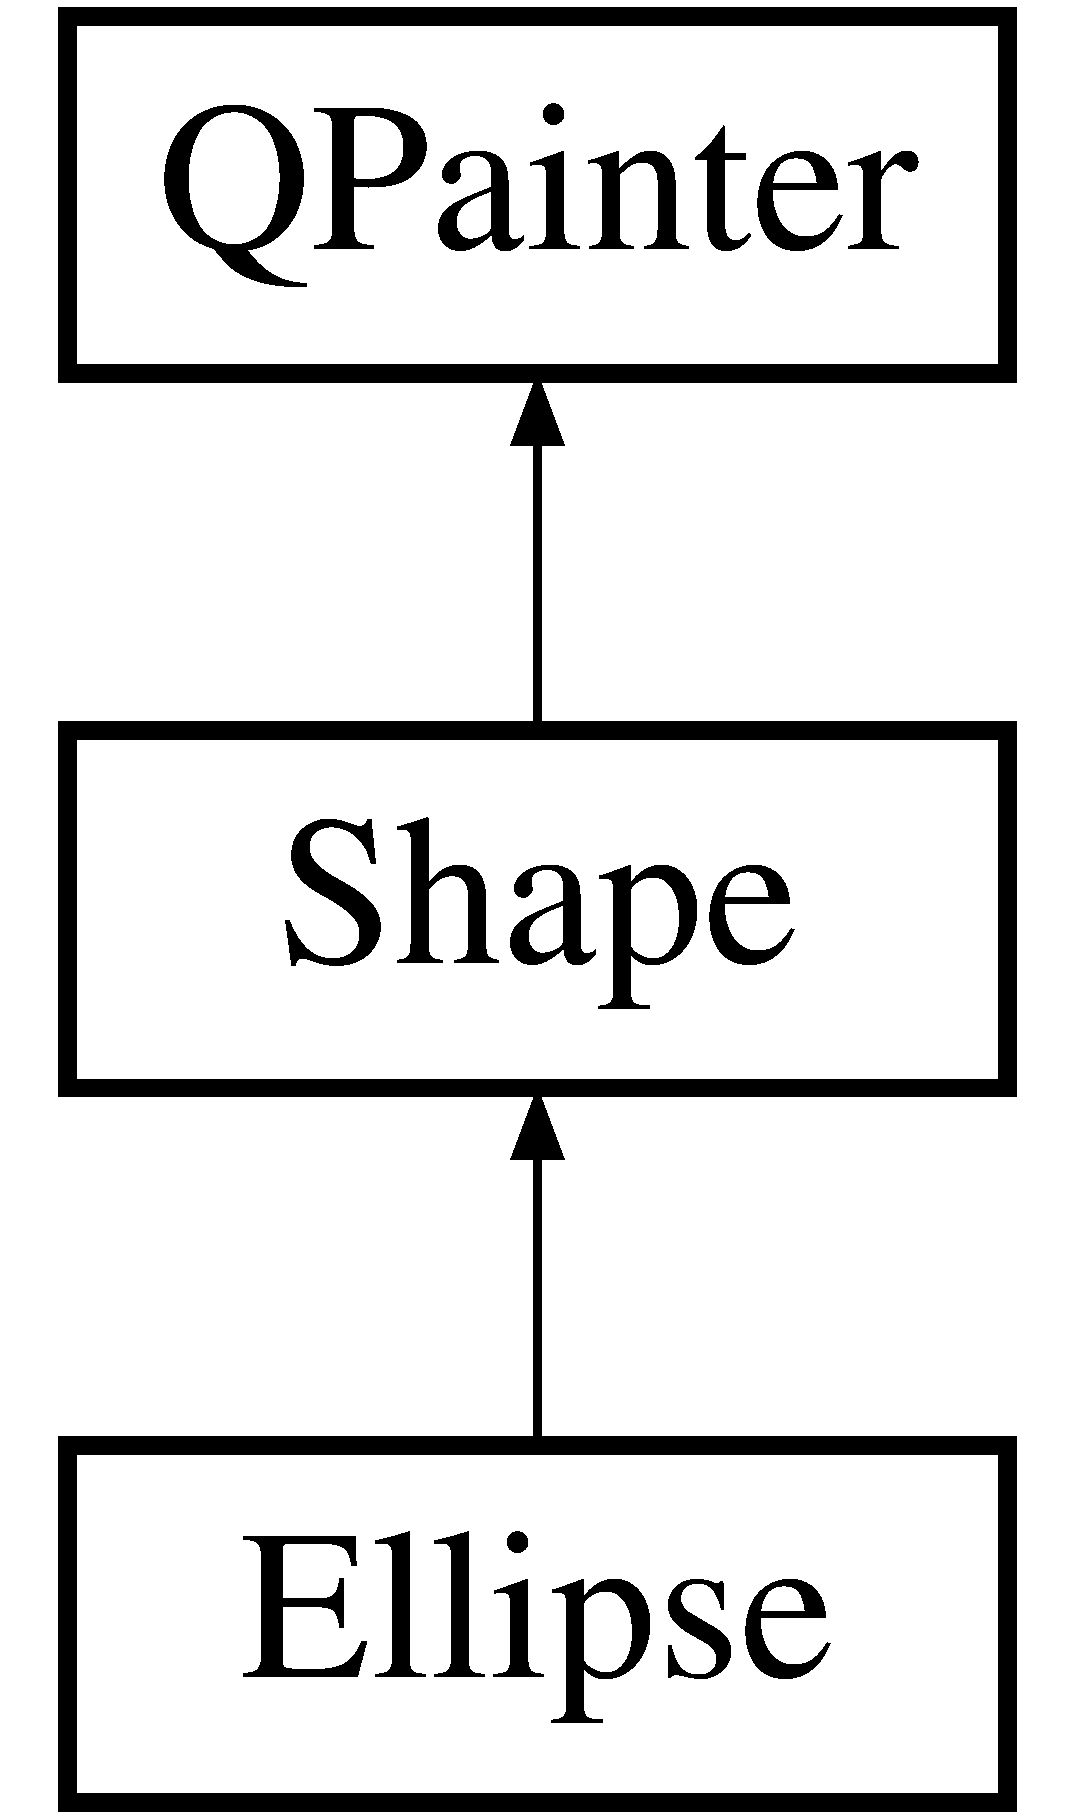
\includegraphics[height=3.000000cm]{class_ellipse}
\end{center}
\end{figure}
\subsection*{Public Member Functions}
\begin{DoxyCompactItemize}
\item 
{\bf Ellipse} (Q\+Paint\+Device $\ast$device=nullptr, int id=-\/1)
\begin{DoxyCompactList}\small\item\em \doxyref{Ellipse}{p.}{class_ellipse} Class constructor. \end{DoxyCompactList}\item 
{\bf $\sim$\+Ellipse} () override\label{class_ellipse_af7b546b29a2f8ce3494f9d02143a621c}

\begin{DoxyCompactList}\small\item\em \doxyref{Ellipse}{p.}{class_ellipse} Class destructor. \end{DoxyCompactList}\item 
void {\bf move} (int x, int y, int na) override
\begin{DoxyCompactList}\small\item\em move function to move an ellipse \end{DoxyCompactList}\item 
void {\bf draw} (Q\+Paint\+Device $\ast$device) override
\begin{DoxyCompactList}\small\item\em draw function to draw an ellipse \end{DoxyCompactList}\item 
double {\bf area} () override
\begin{DoxyCompactList}\small\item\em area function to calculate area of ellipse \end{DoxyCompactList}\item 
double {\bf perimeter} () override
\begin{DoxyCompactList}\small\item\em perimeter function to calculate perimeter of ellipse \end{DoxyCompactList}\item 
double {\bf get\+Width} ()\label{class_ellipse_a79b45a55a6dc182866659c00535bba5e}

\begin{DoxyCompactList}\small\item\em get\+Width function for ellipse class, function returns a double width \end{DoxyCompactList}\item 
double {\bf get\+Height} ()\label{class_ellipse_acd5005522d00f0e3235a2d4d931c0e39}

\begin{DoxyCompactList}\small\item\em get\+Height function for ellipse class, function returns a double height \end{DoxyCompactList}\item 
Q\+Point \& {\bf get\+Location} ()\label{class_ellipse_a39951db608b73cb66b250e2811680faf}

\begin{DoxyCompactList}\small\item\em get\+Location function for ellipse class, function returns a Q\+Point location \end{DoxyCompactList}\item 
void {\bf set\+Dimensions} (double w, double h)
\begin{DoxyCompactList}\small\item\em set\+Dimensions function for ellipse \end{DoxyCompactList}\item 
void {\bf set\+Location} (int x, int y)
\begin{DoxyCompactList}\small\item\em set\+Location function for ellipse \end{DoxyCompactList}\item 
void {\bf set\+Location} (Q\+Point pt)
\begin{DoxyCompactList}\small\item\em set\+Location function for ellipse \end{DoxyCompactList}\end{DoxyCompactItemize}
\subsection*{Additional Inherited Members}


\subsection{Detailed Description}
\doxyref{Ellipse}{p.}{class_ellipse} Class\+: Public Inheritance from \doxyref{Shape}{p.}{class_shape} Class. 

\subsection{Constructor \& Destructor Documentation}
\index{Ellipse@{Ellipse}!Ellipse@{Ellipse}}
\index{Ellipse@{Ellipse}!Ellipse@{Ellipse}}
\subsubsection[{Ellipse(\+Q\+Paint\+Device $\ast$device=nullptr, int id=-\/1)}]{\setlength{\rightskip}{0pt plus 5cm}Ellipse\+::\+Ellipse (
\begin{DoxyParamCaption}
\item[{Q\+Paint\+Device $\ast$}]{device = {\ttfamily nullptr}, }
\item[{int}]{id = {\ttfamily -\/1}}
\end{DoxyParamCaption}
)}\label{class_ellipse_af31f4f441414671f76c60b03516eb5d6}


\doxyref{Ellipse}{p.}{class_ellipse} Class constructor. 

\doxyref{Ellipse}{p.}{class_ellipse} constructor requires two parameters. 
\begin{DoxyParams}{Parameters}
{\em $\ast$device} & is a pointer of type Q\+Paint\+Device, initialized to nullptr to avoid conflict \\
\hline
{\em id} & is of type int \\
\hline
\end{DoxyParams}


\subsection{Member Function Documentation}
\index{Ellipse@{Ellipse}!area@{area}}
\index{area@{area}!Ellipse@{Ellipse}}
\subsubsection[{area() override}]{\setlength{\rightskip}{0pt plus 5cm}double Ellipse\+::area (
\begin{DoxyParamCaption}
{}
\end{DoxyParamCaption}
)\hspace{0.3cm}{\ttfamily [override]}, {\ttfamily [virtual]}}\label{class_ellipse_abdcc9bf2ca75e53000eecd7fce16d1ea}


area function to calculate area of ellipse 

area function overrides the virtual area function of abstract base class shape. Function returns a double. No parameters are passed into area. 

Implements {\bf Shape} \doxyref{}{p.}{class_shape_aa3072fde001d5174f78fcc484c11870c}.

\index{Ellipse@{Ellipse}!draw@{draw}}
\index{draw@{draw}!Ellipse@{Ellipse}}
\subsubsection[{draw(\+Q\+Paint\+Device $\ast$device) override}]{\setlength{\rightskip}{0pt plus 5cm}void Ellipse\+::draw (
\begin{DoxyParamCaption}
\item[{Q\+Paint\+Device $\ast$}]{device}
\end{DoxyParamCaption}
)\hspace{0.3cm}{\ttfamily [override]}, {\ttfamily [virtual]}}\label{class_ellipse_ae83718bf96925955fa48c14a4217c73c}


draw function to draw an ellipse 

draw function overrides the virtual draw from abstract base class shape. Funtion does not return any type. 
\begin{DoxyParams}{Parameters}
{\em $\ast$device} & is a pointer of type Q\+Paint\+Device \\
\hline
\end{DoxyParams}


Implements {\bf Shape} \doxyref{}{p.}{class_shape_ad2ab549a1b0cc0e23af8be1fd1b61a1b}.

\index{Ellipse@{Ellipse}!move@{move}}
\index{move@{move}!Ellipse@{Ellipse}}
\subsubsection[{move(int x, int y, int na) override}]{\setlength{\rightskip}{0pt plus 5cm}void Ellipse\+::move (
\begin{DoxyParamCaption}
\item[{int}]{x, }
\item[{int}]{y, }
\item[{int}]{na}
\end{DoxyParamCaption}
)\hspace{0.3cm}{\ttfamily [override]}, {\ttfamily [virtual]}}\label{class_ellipse_a1929dda25f9dc816835e05c57937d34a}


move function to move an ellipse 

move function overrides the virtual move from abstract base class \doxyref{Shape}{p.}{class_shape}. Function does not return any type. 
\begin{DoxyParams}{Parameters}
{\em x} & is of type int \\
\hline
{\em y} & is of type int \\
\hline
{\em na} & is of type int \\
\hline
\end{DoxyParams}


Implements {\bf Shape} \doxyref{}{p.}{class_shape_a937ef09c5e1c5c640fdef7caf62ba8f2}.

\index{Ellipse@{Ellipse}!perimeter@{perimeter}}
\index{perimeter@{perimeter}!Ellipse@{Ellipse}}
\subsubsection[{perimeter() override}]{\setlength{\rightskip}{0pt plus 5cm}double Ellipse\+::perimeter (
\begin{DoxyParamCaption}
{}
\end{DoxyParamCaption}
)\hspace{0.3cm}{\ttfamily [override]}, {\ttfamily [virtual]}}\label{class_ellipse_abb2c4bca7f3c88c16a81f6ecb9d93e5c}


perimeter function to calculate perimeter of ellipse 

perimeter function overrides the virtual perimeter function of abstract base class shape. Function returns a double. No parameters are passed into area. 

Implements {\bf Shape} \doxyref{}{p.}{class_shape_afb064edd78952da66801619338e8c5a3}.

\index{Ellipse@{Ellipse}!set\+Dimensions@{set\+Dimensions}}
\index{set\+Dimensions@{set\+Dimensions}!Ellipse@{Ellipse}}
\subsubsection[{set\+Dimensions(double w, double h)}]{\setlength{\rightskip}{0pt plus 5cm}void Ellipse\+::set\+Dimensions (
\begin{DoxyParamCaption}
\item[{double}]{w, }
\item[{double}]{h}
\end{DoxyParamCaption}
)}\label{class_ellipse_af3e06272b3d22f3249ff04288df1f6dd}


set\+Dimensions function for ellipse 

set\+Dimensions function requires two parameters. The class member variables width and height are set from these parameters. 
\begin{DoxyParams}{Parameters}
{\em w} & is of type double \\
\hline
{\em h} & is of type double \\
\hline
\end{DoxyParams}
\index{Ellipse@{Ellipse}!set\+Location@{set\+Location}}
\index{set\+Location@{set\+Location}!Ellipse@{Ellipse}}
\subsubsection[{set\+Location(int x, int y)}]{\setlength{\rightskip}{0pt plus 5cm}void Ellipse\+::set\+Location (
\begin{DoxyParamCaption}
\item[{int}]{x, }
\item[{int}]{y}
\end{DoxyParamCaption}
)}\label{class_ellipse_aa24fd99eedbfc4b45c2b2c2a11cd5759}


set\+Location function for ellipse 

set\+Location function requires two arguments. Takes the two arguments and makes a coordinate pair (Q\+Point) consisting of these values. 
\begin{DoxyParams}{Parameters}
{\em x} & is of type int \\
\hline
{\em y} & is of type int \\
\hline
\end{DoxyParams}
\index{Ellipse@{Ellipse}!set\+Location@{set\+Location}}
\index{set\+Location@{set\+Location}!Ellipse@{Ellipse}}
\subsubsection[{set\+Location(\+Q\+Point pt)}]{\setlength{\rightskip}{0pt plus 5cm}void Ellipse\+::set\+Location (
\begin{DoxyParamCaption}
\item[{Q\+Point}]{pt}
\end{DoxyParamCaption}
)}\label{class_ellipse_a4af4a28871b606d434fc62aee9f82c24}


set\+Location function for ellipse 

set\+Location function requires a single parameter. The class memeber variable location is set to the Q\+Point parameter passed in. 
\begin{DoxyParams}{Parameters}
{\em pt} & is of type Q\+Point \\
\hline
\end{DoxyParams}


The documentation for this class was generated from the following file\+:\begin{DoxyCompactItemize}
\item 
Shape.\+h\end{DoxyCompactItemize}

\section{Line Class Reference}
\label{class_line}\index{Line@{Line}}


\doxyref{Line}{p.}{class_line} Class\+: Public Inheritance from \doxyref{Shape}{p.}{class_shape} Class.  




{\ttfamily \#include $<$Shape.\+h$>$}

Inheritance diagram for Line\+:\begin{figure}[H]
\begin{center}
\leavevmode
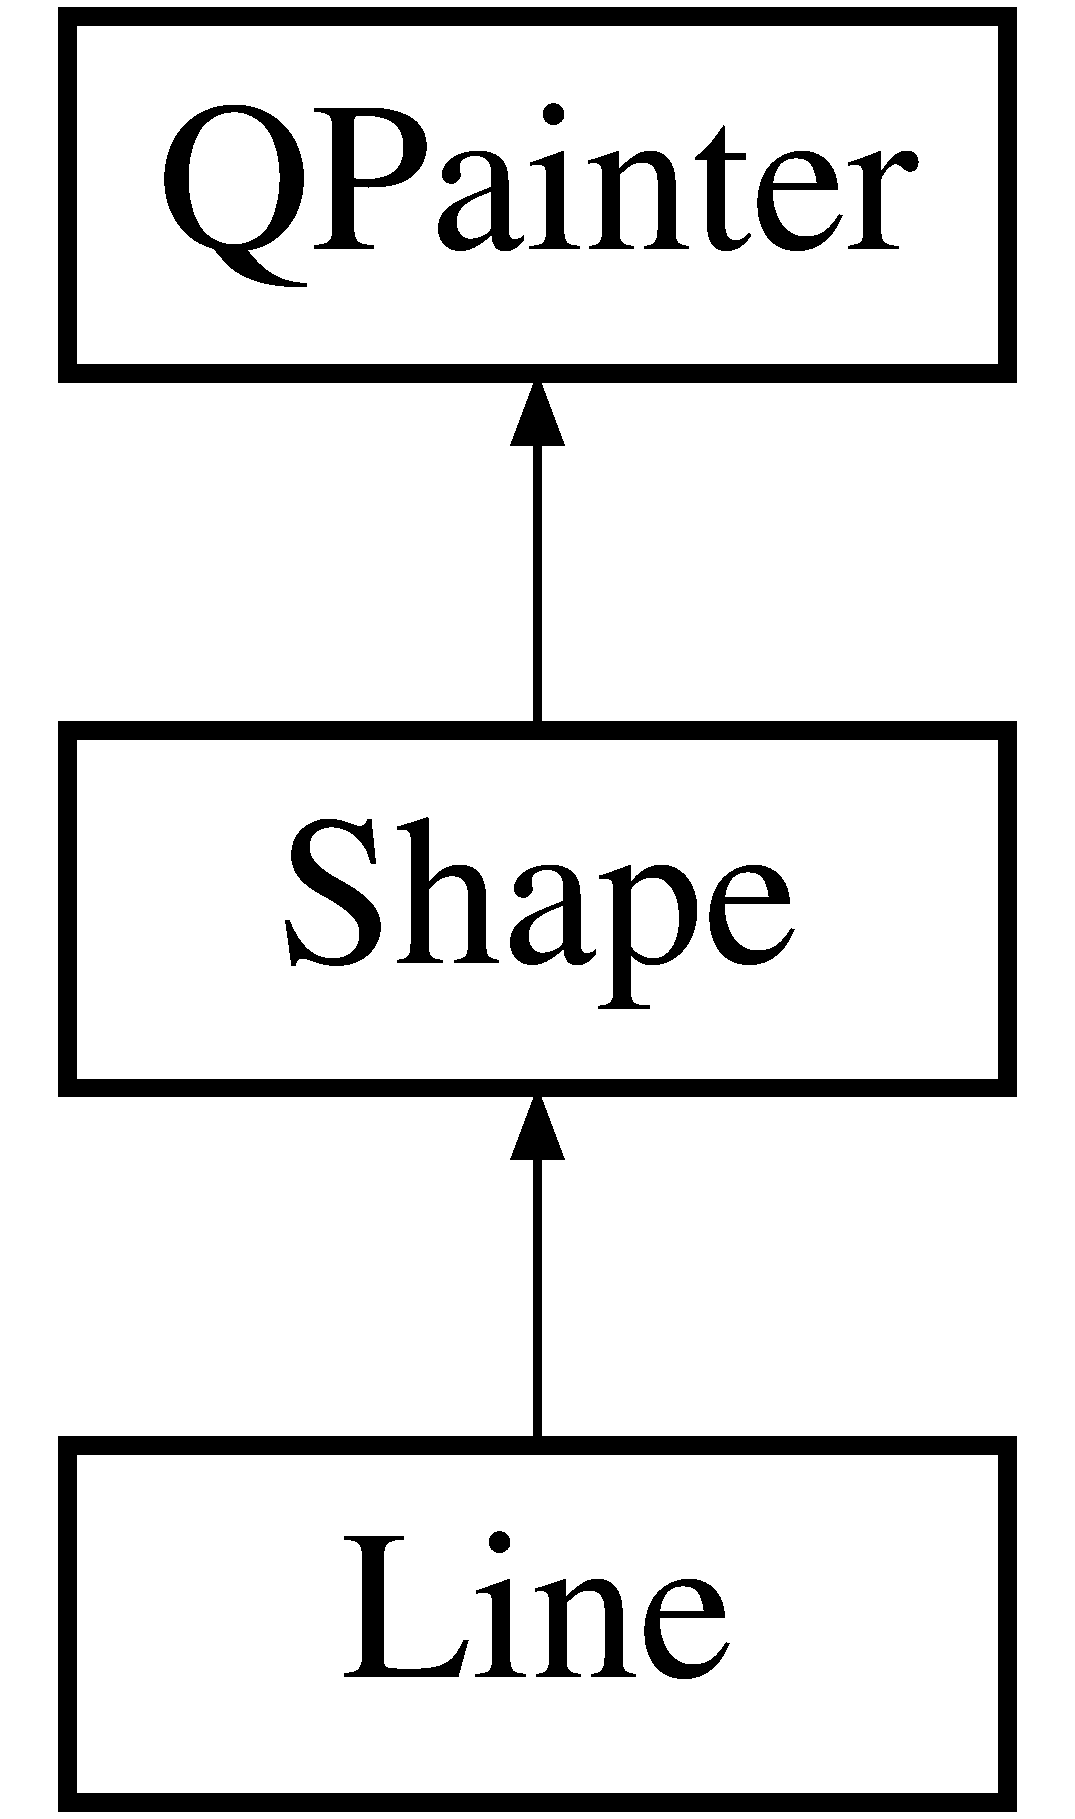
\includegraphics[height=3.000000cm]{class_line}
\end{center}
\end{figure}
\subsection*{Public Member Functions}
\begin{DoxyCompactItemize}
\item 
{\bf Line} (Q\+Paint\+Device $\ast$device=nullptr, int id=-\/1)
\begin{DoxyCompactList}\small\item\em \doxyref{Line}{p.}{class_line} Class Constructor. \end{DoxyCompactList}\item 
{\bf $\sim$\+Line} () override\label{class_line_af18447238883377a0071d2276a4ac0a5}

\begin{DoxyCompactList}\small\item\em \doxyref{Line}{p.}{class_line} Class Destructor. \end{DoxyCompactList}\item 
void {\bf set\+Points} (const Q\+Point \&x, const Q\+Point \&y)
\begin{DoxyCompactList}\small\item\em set\+Points function for \doxyref{Line}{p.}{class_line} \end{DoxyCompactList}\item 
virtual void {\bf move} (const int x, const int y, int vert) override
\begin{DoxyCompactList}\small\item\em move function to move a line \end{DoxyCompactList}\item 
virtual void {\bf draw} (Q\+Paint\+Device $\ast$device) override
\begin{DoxyCompactList}\small\item\em draw function to draw a line \end{DoxyCompactList}\item 
virtual double {\bf perimeter} () override
\begin{DoxyCompactList}\small\item\em perimeter function to calculate perimeter of a line \end{DoxyCompactList}\item 
virtual double {\bf area} () override
\begin{DoxyCompactList}\small\item\em area function to calculate area of a line \end{DoxyCompactList}\end{DoxyCompactItemize}
\subsection*{Additional Inherited Members}


\subsection{Detailed Description}
\doxyref{Line}{p.}{class_line} Class\+: Public Inheritance from \doxyref{Shape}{p.}{class_shape} Class. 

\subsection{Constructor \& Destructor Documentation}
\index{Line@{Line}!Line@{Line}}
\index{Line@{Line}!Line@{Line}}
\subsubsection[{Line(\+Q\+Paint\+Device $\ast$device=nullptr, int id=-\/1)}]{\setlength{\rightskip}{0pt plus 5cm}Line\+::\+Line (
\begin{DoxyParamCaption}
\item[{Q\+Paint\+Device $\ast$}]{device = {\ttfamily nullptr}, }
\item[{int}]{id = {\ttfamily -\/1}}
\end{DoxyParamCaption}
)}\label{class_line_abfce044bd32535d51e49ed00d401aee0}


\doxyref{Line}{p.}{class_line} Class Constructor. 

\doxyref{Line}{p.}{class_line} Class constructor takes in two parameters 
\begin{DoxyParams}{Parameters}
{\em $\ast$device} & is a pointer of type Q\+Paint\+Device, initialized to nullptr to avoid conflicts \\
\hline
{\em id} & is of type int \\
\hline
\end{DoxyParams}


\subsection{Member Function Documentation}
\index{Line@{Line}!area@{area}}
\index{area@{area}!Line@{Line}}
\subsubsection[{area() override}]{\setlength{\rightskip}{0pt plus 5cm}virtual double Line\+::area (
\begin{DoxyParamCaption}
{}
\end{DoxyParamCaption}
)\hspace{0.3cm}{\ttfamily [inline]}, {\ttfamily [override]}, {\ttfamily [virtual]}}\label{class_line_a5989f939ab0025b09d0da1aee6421122}


area function to calculate area of a line 

area function overrides the virtual area function of abstract base class shape. Function returns a double. No parameters are passed into area, line does not have area so the function is defined only by \char`\"{}return 0\char`\"{}. Function definition must be defined as return 0, else line class will be recognized as an abstract class. 

Implements {\bf Shape} \doxyref{}{p.}{class_shape_aa3072fde001d5174f78fcc484c11870c}.

\index{Line@{Line}!draw@{draw}}
\index{draw@{draw}!Line@{Line}}
\subsubsection[{draw(\+Q\+Paint\+Device $\ast$device) override}]{\setlength{\rightskip}{0pt plus 5cm}virtual void Line\+::draw (
\begin{DoxyParamCaption}
\item[{Q\+Paint\+Device $\ast$}]{device}
\end{DoxyParamCaption}
)\hspace{0.3cm}{\ttfamily [override]}, {\ttfamily [virtual]}}\label{class_line_a3b191dfa5dd12e9be51ed225607696e5}


draw function to draw a line 

draw function overrides the virtual draw from abstract base class shape. Funtion does not return any type. 
\begin{DoxyParams}{Parameters}
{\em $\ast$device} & is a pointer of type Q\+Paint\+Device \\
\hline
\end{DoxyParams}


Implements {\bf Shape} \doxyref{}{p.}{class_shape_ad2ab549a1b0cc0e23af8be1fd1b61a1b}.

\index{Line@{Line}!move@{move}}
\index{move@{move}!Line@{Line}}
\subsubsection[{move(const int x, const int y, int vert) override}]{\setlength{\rightskip}{0pt plus 5cm}virtual void Line\+::move (
\begin{DoxyParamCaption}
\item[{const int}]{x, }
\item[{const int}]{y, }
\item[{int}]{vert}
\end{DoxyParamCaption}
)\hspace{0.3cm}{\ttfamily [override]}, {\ttfamily [virtual]}}\label{class_line_abbae60ea00ae0759ede7b43b788c2028}


move function to move a line 

move function overrides the virtual move from abstract base class \doxyref{Shape}{p.}{class_shape}. Function does not return any type. 
\begin{DoxyParams}{Parameters}
{\em x} & is of type constant int \\
\hline
{\em y} & is of type constant int \\
\hline
{\em vert} & is of type int \\
\hline
\end{DoxyParams}


Implements {\bf Shape} \doxyref{}{p.}{class_shape_a937ef09c5e1c5c640fdef7caf62ba8f2}.

\index{Line@{Line}!perimeter@{perimeter}}
\index{perimeter@{perimeter}!Line@{Line}}
\subsubsection[{perimeter() override}]{\setlength{\rightskip}{0pt plus 5cm}virtual double Line\+::perimeter (
\begin{DoxyParamCaption}
{}
\end{DoxyParamCaption}
)\hspace{0.3cm}{\ttfamily [inline]}, {\ttfamily [override]}, {\ttfamily [virtual]}}\label{class_line_ad1fa30c56b29c961f26885edcb2f8109}


perimeter function to calculate perimeter of a line 

perimeter function overrides the virtual perimeter function of abstract base class shape. Function returns a double. No parameters are passed into perimeter, line does not have perimeter so the function is defined only by \char`\"{}return 0\char`\"{}. Function definition must be defined as return 0, else line class will be recognized as an abstract class. 

Implements {\bf Shape} \doxyref{}{p.}{class_shape_afb064edd78952da66801619338e8c5a3}.

\index{Line@{Line}!set\+Points@{set\+Points}}
\index{set\+Points@{set\+Points}!Line@{Line}}
\subsubsection[{set\+Points(const Q\+Point \&x, const Q\+Point \&y)}]{\setlength{\rightskip}{0pt plus 5cm}void Line\+::set\+Points (
\begin{DoxyParamCaption}
\item[{const Q\+Point \&}]{x, }
\item[{const Q\+Point \&}]{y}
\end{DoxyParamCaption}
)\hspace{0.3cm}{\ttfamily [inline]}}\label{class_line_a1ff33e610802339eca8d9b421b32dd60}


set\+Points function for \doxyref{Line}{p.}{class_line} 

set\+Points function allows the line to be set with given starting and ending points The class member variables line\+\_\+begin and line\+\_\+end are set to parameters x,y 
\begin{DoxyParams}{Parameters}
{\em x} & is a constant reference of type Q\+Point \\
\hline
{\em y} & is a constant reference of type Q\+Point \\
\hline
\end{DoxyParams}


The documentation for this class was generated from the following file\+:\begin{DoxyCompactItemize}
\item 
Shape.\+h\end{DoxyCompactItemize}

\section{Main\+Window Class Reference}
\label{class_main_window}\index{Main\+Window@{Main\+Window}}


\doxyref{Main\+Window}{p.}{class_main_window} Class\+: Public Inheritance from Q\+Main\+Window.  




{\ttfamily \#include $<$mainwindow.\+h$>$}

Inheritance diagram for Main\+Window\+:\begin{figure}[H]
\begin{center}
\leavevmode
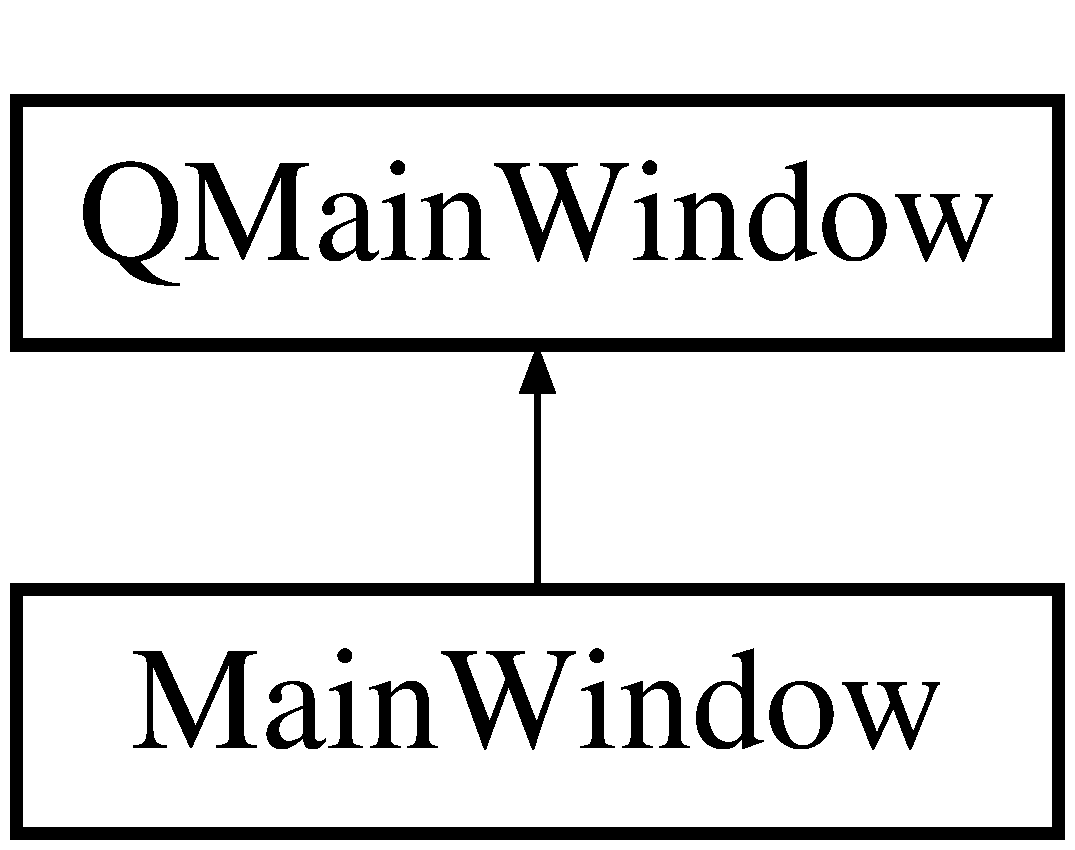
\includegraphics[height=2.000000cm]{class_main_window}
\end{center}
\end{figure}
\subsection*{Public Member Functions}
\begin{DoxyCompactItemize}
\item 
{\bf Main\+Window} (Q\+Widget $\ast$parent=nullptr)
\begin{DoxyCompactList}\small\item\em Main Window Contructor. \end{DoxyCompactList}\item 
{\bf $\sim$\+Main\+Window} ()\label{class_main_window_ae98d00a93bc118200eeef9f9bba1dba7}

\begin{DoxyCompactList}\small\item\em Destructor for \doxyref{Main\+Window}{p.}{class_main_window}. \end{DoxyCompactList}\item 
void {\bfseries allow\+Meddling} (bool YN)\label{class_main_window_a4523d1c1de1c700095daf9cd76e42674}

\item 
void {\bf get\+Shape\+Type} (Q\+Combo\+Box $\ast$combo)
\begin{DoxyCompactList}\small\item\em get\+Shape\+Type function for \doxyref{Main\+Window}{p.}{class_main_window} \end{DoxyCompactList}\item 
void {\bf get\+Pen\+Color} (Q\+Combo\+Box $\ast$combo)\label{class_main_window_a963a89531d8ef7a819934885c0658d23}

\begin{DoxyCompactList}\small\item\em get\+Pen\+Color function for \doxyref{Main\+Window}{p.}{class_main_window} \end{DoxyCompactList}\item 
void {\bf get\+Pen\+Style} (Q\+Combo\+Box $\ast$combo)\label{class_main_window_af2c5ffffeca69641c5c9370a5450323e}

\begin{DoxyCompactList}\small\item\em get\+Pen\+Style function for \doxyref{Main\+Window}{p.}{class_main_window} \end{DoxyCompactList}\item 
void {\bf get\+Pen\+Cap\+Style} (Q\+Combo\+Box $\ast$combo)\label{class_main_window_aaee7a5858cdeff3c6919a2b1f1dcd8a8}

\begin{DoxyCompactList}\small\item\em get\+Pen\+Cap\+Style function for \doxyref{Main\+Window}{p.}{class_main_window} \end{DoxyCompactList}\item 
void {\bf get\+Pen\+Join\+Style} (Q\+Combo\+Box $\ast$combo)\label{class_main_window_a5eb82c6e6db6b6569f228ba1c024c04e}

\begin{DoxyCompactList}\small\item\em get\+Pen\+Join\+Style function for \doxyref{Main\+Window}{p.}{class_main_window} \end{DoxyCompactList}\item 
void {\bf get\+Brush\+Color} (Q\+Combo\+Box $\ast$combo)\label{class_main_window_af7641d85fa0a8c445ca1ddc58b0a7e33}

\begin{DoxyCompactList}\small\item\em get\+Brush\+Color function for \doxyref{Main\+Window}{p.}{class_main_window} \end{DoxyCompactList}\item 
void {\bf get\+Brush\+Style} (Q\+Combo\+Box $\ast$combo)\label{class_main_window_a42e32bde778e58e9fdef8f9230ad988f}

\begin{DoxyCompactList}\small\item\em get\+Brush\+Style function for \doxyref{Main\+Window}{p.}{class_main_window} \end{DoxyCompactList}\item 
Qt\+::\+Alignment\+Flag {\bf get\+Align} (Q\+Combo\+Box $\ast$combo)
\begin{DoxyCompactList}\small\item\em get\+Align function for \doxyref{Main\+Window}{p.}{class_main_window} \end{DoxyCompactList}\item 
Qt\+::\+Global\+Color {\bf get\+Text\+Color} (Q\+Combo\+Box $\ast$combo)
\begin{DoxyCompactList}\small\item\em get\+Text\+Color function for \doxyref{Main\+Window}{p.}{class_main_window} \end{DoxyCompactList}\item 
Q\+Font\+::\+Weight {\bf get\+Text\+Weight} (Q\+Combo\+Box $\ast$combo)
\begin{DoxyCompactList}\small\item\em get\+Text\+Weight function for \doxyref{Main\+Window}{p.}{class_main_window} \end{DoxyCompactList}\item 
Q\+Font\+::\+Style {\bf get\+Text\+Style} (Q\+Combo\+Box $\ast$combo)
\begin{DoxyCompactList}\small\item\em get\+Text\+Style function for \doxyref{Main\+Window}{p.}{class_main_window} \end{DoxyCompactList}\item 
Q\+String {\bf get\+Font\+Family} (Q\+Combo\+Box $\ast$combo)
\begin{DoxyCompactList}\small\item\em get\+Font\+Family function for \doxyref{Main\+Window}{p.}{class_main_window} \end{DoxyCompactList}\item 
void {\bfseries get\+Pen\+Width} (Q\+Spin\+Box $\ast$spinster)\label{class_main_window_a93e2ced16f27f6e85e8f8cdb93415199}

\item 
void {\bf set\+Shape\+Nonsense} ({\bf Shape} $\ast$shape, {\bf Shape\+::\+Shape\+Type}, int id, Qt\+::\+Global\+Color pc, int pw, Qt\+::\+Pen\+Style ps, Qt\+::\+Pen\+Cap\+Style pcs, Qt\+::\+Pen\+Join\+Style pjs, Qt\+::\+Global\+Color bc, Qt\+::\+Brush\+Style bs)
\begin{DoxyCompactList}\small\item\em set\+Shape\+Nonsense function for \doxyref{Main\+Window}{p.}{class_main_window} \end{DoxyCompactList}\item 
void {\bf combo\+Trick\+Colors} (Q\+Combo\+Box $\ast$combo)
\begin{DoxyCompactList}\small\item\em combo\+Trick\+Colors function for \doxyref{Main\+Window}{p.}{class_main_window} \end{DoxyCompactList}\item 
void {\bf combo\+Trick\+Shapes} (Q\+Combo\+Box $\ast$combo)
\begin{DoxyCompactList}\small\item\em combo\+Trick\+Shapes function for \doxyref{Main\+Window}{p.}{class_main_window} \end{DoxyCompactList}\item 
void {\bf combo\+Trick\+Pen\+Styles} (Q\+Combo\+Box $\ast$combo)
\begin{DoxyCompactList}\small\item\em combo\+Trick\+Pen\+Styles function for \doxyref{Main\+Window}{p.}{class_main_window} \end{DoxyCompactList}\item 
void {\bf combo\+Trick\+Pen\+Cap\+Styles} (Q\+Combo\+Box $\ast$combo)
\begin{DoxyCompactList}\small\item\em combo\+Trick\+Pen\+Cap\+Styles function for \doxyref{Main\+Window}{p.}{class_main_window} \end{DoxyCompactList}\item 
void {\bf combo\+Trick\+Pen\+Join\+Styles} (Q\+Combo\+Box $\ast$combo)
\begin{DoxyCompactList}\small\item\em combo\+Trick\+Pen\+Join\+Styles function for \doxyref{Main\+Window}{p.}{class_main_window} \end{DoxyCompactList}\item 
void {\bf combo\+Trick\+Bush\+Style} (Q\+Combo\+Box $\ast$combo)
\begin{DoxyCompactList}\small\item\em combo\+Trick\+Bush\+Style function for \doxyref{Main\+Window}{p.}{class_main_window} \end{DoxyCompactList}\item 
void {\bf combo\+Trick\+Flag} (Q\+Combo\+Box $\ast$combo)
\begin{DoxyCompactList}\small\item\em combo\+Trick\+Flag function for \doxyref{Main\+Window}{p.}{class_main_window} \end{DoxyCompactList}\item 
void {\bf combo\+Trick\+Font\+Style} (Q\+Combo\+Box $\ast$combo)
\begin{DoxyCompactList}\small\item\em combo\+Trick\+Font\+Style function for \doxyref{Main\+Window}{p.}{class_main_window} \end{DoxyCompactList}\item 
void {\bf combo\+Trick\+Font\+Fam} (Q\+Combo\+Box $\ast$combo)
\begin{DoxyCompactList}\small\item\em combo\+Trick\+Font\+Fam function for \doxyref{Main\+Window}{p.}{class_main_window} \end{DoxyCompactList}\item 
void {\bf combo\+Trick\+Font\+Weight} (Q\+Combo\+Box $\ast$combo)
\begin{DoxyCompactList}\small\item\em combo\+Trick\+Font\+Weight function for \doxyref{Main\+Window}{p.}{class_main_window} \end{DoxyCompactList}\item 
void {\bfseries debug\+Print\+Shape\+Info} ()\label{class_main_window_abb5f4cadb1eda28c22883166400b38cf}

\end{DoxyCompactItemize}


\subsection{Detailed Description}
\doxyref{Main\+Window}{p.}{class_main_window} Class\+: Public Inheritance from Q\+Main\+Window. 

Q\+Main\+Window provides a main application window. This mainwindow provides a framework for building an apllication based user interface. \doxyref{Main\+Window}{p.}{class_main_window} adds additional features to Q\+Main\+Window with the use of Q\+Combo\+Box and Q\+Spin\+Box. 

\subsection{Constructor \& Destructor Documentation}
\index{Main\+Window@{Main\+Window}!Main\+Window@{Main\+Window}}
\index{Main\+Window@{Main\+Window}!Main\+Window@{Main\+Window}}
\subsubsection[{Main\+Window(\+Q\+Widget $\ast$parent=nullptr)}]{\setlength{\rightskip}{0pt plus 5cm}Main\+Window\+::\+Main\+Window (
\begin{DoxyParamCaption}
\item[{Q\+Widget $\ast$}]{parent = {\ttfamily nullptr}}
\end{DoxyParamCaption}
)\hspace{0.3cm}{\ttfamily [explicit]}}\label{class_main_window_a996c5a2b6f77944776856f08ec30858d}


Main Window Contructor. 

Constructs a \doxyref{Main\+Window}{p.}{class_main_window} using a pointer of type Q\+Widget, which is the base class of user interface objects (receives keyboard, mouse, and other events to draw images). 

\subsection{Member Function Documentation}
\index{Main\+Window@{Main\+Window}!combo\+Trick\+Bush\+Style@{combo\+Trick\+Bush\+Style}}
\index{combo\+Trick\+Bush\+Style@{combo\+Trick\+Bush\+Style}!Main\+Window@{Main\+Window}}
\subsubsection[{combo\+Trick\+Bush\+Style(\+Q\+Combo\+Box $\ast$combo)}]{\setlength{\rightskip}{0pt plus 5cm}void Main\+Window\+::combo\+Trick\+Bush\+Style (
\begin{DoxyParamCaption}
\item[{Q\+Combo\+Box $\ast$}]{combo}
\end{DoxyParamCaption}
)}\label{class_main_window_aed392f373a13584ce3b0e71f31fe069a}


combo\+Trick\+Bush\+Style function for \doxyref{Main\+Window}{p.}{class_main_window} 

combo\+Trick\+Bush\+Style function adds a drop down menu for brush style on the main window. Q\+Combo\+Box pointer required as a paramter. No value or reference is returned. 
\begin{DoxyParams}{Parameters}
{\em combo} & is a pointer of type Q\+Combo\+Box \\
\hline
\end{DoxyParams}
\index{Main\+Window@{Main\+Window}!combo\+Trick\+Colors@{combo\+Trick\+Colors}}
\index{combo\+Trick\+Colors@{combo\+Trick\+Colors}!Main\+Window@{Main\+Window}}
\subsubsection[{combo\+Trick\+Colors(\+Q\+Combo\+Box $\ast$combo)}]{\setlength{\rightskip}{0pt plus 5cm}void Main\+Window\+::combo\+Trick\+Colors (
\begin{DoxyParamCaption}
\item[{Q\+Combo\+Box $\ast$}]{combo}
\end{DoxyParamCaption}
)}\label{class_main_window_a4521bf4cbf18590dbf4f18b8a883a833}


combo\+Trick\+Colors function for \doxyref{Main\+Window}{p.}{class_main_window} 

combo\+Trick\+Colors function adds a drop down menu for colors on the main window. Q\+Combo\+Box pointer required as a paramter. No value or reference is returned. 
\begin{DoxyParams}{Parameters}
{\em combo} & is a pointer of type Q\+Combo\+Box \\
\hline
\end{DoxyParams}
\index{Main\+Window@{Main\+Window}!combo\+Trick\+Flag@{combo\+Trick\+Flag}}
\index{combo\+Trick\+Flag@{combo\+Trick\+Flag}!Main\+Window@{Main\+Window}}
\subsubsection[{combo\+Trick\+Flag(\+Q\+Combo\+Box $\ast$combo)}]{\setlength{\rightskip}{0pt plus 5cm}void Main\+Window\+::combo\+Trick\+Flag (
\begin{DoxyParamCaption}
\item[{Q\+Combo\+Box $\ast$}]{combo}
\end{DoxyParamCaption}
)}\label{class_main_window_ace09a5740d9079a0e48551f616ab1846}


combo\+Trick\+Flag function for \doxyref{Main\+Window}{p.}{class_main_window} 

combo\+Trick\+Flag function adds a drop down menu for flags on the main window. Q\+Combo\+Box pointer required as a paramter. No value or reference is returned. 
\begin{DoxyParams}{Parameters}
{\em combo} & is a pointer of type Q\+Combo\+Box \\
\hline
\end{DoxyParams}
\index{Main\+Window@{Main\+Window}!combo\+Trick\+Font\+Fam@{combo\+Trick\+Font\+Fam}}
\index{combo\+Trick\+Font\+Fam@{combo\+Trick\+Font\+Fam}!Main\+Window@{Main\+Window}}
\subsubsection[{combo\+Trick\+Font\+Fam(\+Q\+Combo\+Box $\ast$combo)}]{\setlength{\rightskip}{0pt plus 5cm}void Main\+Window\+::combo\+Trick\+Font\+Fam (
\begin{DoxyParamCaption}
\item[{Q\+Combo\+Box $\ast$}]{combo}
\end{DoxyParamCaption}
)}\label{class_main_window_a7998e234dd35f30cdea8cfd8c9da25ce}


combo\+Trick\+Font\+Fam function for \doxyref{Main\+Window}{p.}{class_main_window} 

combo\+Trick\+Font\+Fam function adds a drop down menu for font families on the main window. Q\+Combo\+Box pointer required as a paramter. No value or reference is returned. 
\begin{DoxyParams}{Parameters}
{\em combo} & is a pointer of type Q\+Combo\+Box \\
\hline
\end{DoxyParams}
\index{Main\+Window@{Main\+Window}!combo\+Trick\+Font\+Style@{combo\+Trick\+Font\+Style}}
\index{combo\+Trick\+Font\+Style@{combo\+Trick\+Font\+Style}!Main\+Window@{Main\+Window}}
\subsubsection[{combo\+Trick\+Font\+Style(\+Q\+Combo\+Box $\ast$combo)}]{\setlength{\rightskip}{0pt plus 5cm}void Main\+Window\+::combo\+Trick\+Font\+Style (
\begin{DoxyParamCaption}
\item[{Q\+Combo\+Box $\ast$}]{combo}
\end{DoxyParamCaption}
)}\label{class_main_window_a51b482222740d86197730ca5c42bb47c}


combo\+Trick\+Font\+Style function for \doxyref{Main\+Window}{p.}{class_main_window} 

combo\+Trick\+Font\+Style function adds a drop down menu for font styles on the main window. Q\+Combo\+Box pointer required as a paramter. No value or reference is returned. 
\begin{DoxyParams}{Parameters}
{\em combo} & is a pointer of type Q\+Combo\+Box \\
\hline
\end{DoxyParams}
\index{Main\+Window@{Main\+Window}!combo\+Trick\+Font\+Weight@{combo\+Trick\+Font\+Weight}}
\index{combo\+Trick\+Font\+Weight@{combo\+Trick\+Font\+Weight}!Main\+Window@{Main\+Window}}
\subsubsection[{combo\+Trick\+Font\+Weight(\+Q\+Combo\+Box $\ast$combo)}]{\setlength{\rightskip}{0pt plus 5cm}void Main\+Window\+::combo\+Trick\+Font\+Weight (
\begin{DoxyParamCaption}
\item[{Q\+Combo\+Box $\ast$}]{combo}
\end{DoxyParamCaption}
)}\label{class_main_window_aef0e18d2b4c06d35f1654e988fe97c74}


combo\+Trick\+Font\+Weight function for \doxyref{Main\+Window}{p.}{class_main_window} 

combo\+Trick\+Font\+Weight function adds a drop down menu for font weights on the main window. Q\+Combo\+Box pointer required as a paramter. No value or reference is returned. 
\begin{DoxyParams}{Parameters}
{\em combo} & is a pointer of type Q\+Combo\+Box \\
\hline
\end{DoxyParams}
\index{Main\+Window@{Main\+Window}!combo\+Trick\+Pen\+Cap\+Styles@{combo\+Trick\+Pen\+Cap\+Styles}}
\index{combo\+Trick\+Pen\+Cap\+Styles@{combo\+Trick\+Pen\+Cap\+Styles}!Main\+Window@{Main\+Window}}
\subsubsection[{combo\+Trick\+Pen\+Cap\+Styles(\+Q\+Combo\+Box $\ast$combo)}]{\setlength{\rightskip}{0pt plus 5cm}void Main\+Window\+::combo\+Trick\+Pen\+Cap\+Styles (
\begin{DoxyParamCaption}
\item[{Q\+Combo\+Box $\ast$}]{combo}
\end{DoxyParamCaption}
)}\label{class_main_window_af739032f27da0957469ec9530fcc6a89}


combo\+Trick\+Pen\+Cap\+Styles function for \doxyref{Main\+Window}{p.}{class_main_window} 

combo\+Trick\+Pen\+Cap\+Styles function adds a drop down menu for pen cap styles on the main window. Q\+Combo\+Box pointer required as a paramter. No value or reference is returned. 
\begin{DoxyParams}{Parameters}
{\em combo} & is a pointer of type Q\+Combo\+Box \\
\hline
\end{DoxyParams}
\index{Main\+Window@{Main\+Window}!combo\+Trick\+Pen\+Join\+Styles@{combo\+Trick\+Pen\+Join\+Styles}}
\index{combo\+Trick\+Pen\+Join\+Styles@{combo\+Trick\+Pen\+Join\+Styles}!Main\+Window@{Main\+Window}}
\subsubsection[{combo\+Trick\+Pen\+Join\+Styles(\+Q\+Combo\+Box $\ast$combo)}]{\setlength{\rightskip}{0pt plus 5cm}void Main\+Window\+::combo\+Trick\+Pen\+Join\+Styles (
\begin{DoxyParamCaption}
\item[{Q\+Combo\+Box $\ast$}]{combo}
\end{DoxyParamCaption}
)}\label{class_main_window_a53f4db98158ef78ead961106e7fa19a0}


combo\+Trick\+Pen\+Join\+Styles function for \doxyref{Main\+Window}{p.}{class_main_window} 

combo\+Trick\+Pen\+Join\+Styles function adds a drop down menu for pen join styles on the main window. Q\+Combo\+Box pointer required as a paramter. No value or reference is returned. 
\begin{DoxyParams}{Parameters}
{\em combo} & is a pointer of type Q\+Combo\+Box \\
\hline
\end{DoxyParams}
\index{Main\+Window@{Main\+Window}!combo\+Trick\+Pen\+Styles@{combo\+Trick\+Pen\+Styles}}
\index{combo\+Trick\+Pen\+Styles@{combo\+Trick\+Pen\+Styles}!Main\+Window@{Main\+Window}}
\subsubsection[{combo\+Trick\+Pen\+Styles(\+Q\+Combo\+Box $\ast$combo)}]{\setlength{\rightskip}{0pt plus 5cm}void Main\+Window\+::combo\+Trick\+Pen\+Styles (
\begin{DoxyParamCaption}
\item[{Q\+Combo\+Box $\ast$}]{combo}
\end{DoxyParamCaption}
)}\label{class_main_window_a60c55e5cb97fdadbdfc1e87a06088aa9}


combo\+Trick\+Pen\+Styles function for \doxyref{Main\+Window}{p.}{class_main_window} 

combo\+Trick\+Pen\+Styles function adds a drop down menu for pen styles on the main window. Q\+Combo\+Box pointer required as a paramter. No value or reference is returned. 
\begin{DoxyParams}{Parameters}
{\em combo} & is a pointer of type Q\+Combo\+Box \\
\hline
\end{DoxyParams}
\index{Main\+Window@{Main\+Window}!combo\+Trick\+Shapes@{combo\+Trick\+Shapes}}
\index{combo\+Trick\+Shapes@{combo\+Trick\+Shapes}!Main\+Window@{Main\+Window}}
\subsubsection[{combo\+Trick\+Shapes(\+Q\+Combo\+Box $\ast$combo)}]{\setlength{\rightskip}{0pt plus 5cm}void Main\+Window\+::combo\+Trick\+Shapes (
\begin{DoxyParamCaption}
\item[{Q\+Combo\+Box $\ast$}]{combo}
\end{DoxyParamCaption}
)}\label{class_main_window_ae4de67e3b1b8cd119e66606b85cf5083}


combo\+Trick\+Shapes function for \doxyref{Main\+Window}{p.}{class_main_window} 

combo\+Trick\+Shapes function adds a drop down menu for shapes on the main window. Q\+Combo\+Box pointer required as a paramter. No value or reference is returned. 
\begin{DoxyParams}{Parameters}
{\em combo} & is a pointer of type Q\+Combo\+Box \\
\hline
\end{DoxyParams}
\index{Main\+Window@{Main\+Window}!get\+Align@{get\+Align}}
\index{get\+Align@{get\+Align}!Main\+Window@{Main\+Window}}
\subsubsection[{get\+Align(\+Q\+Combo\+Box $\ast$combo)}]{\setlength{\rightskip}{0pt plus 5cm}Qt\+::\+Alignment\+Flag Main\+Window\+::get\+Align (
\begin{DoxyParamCaption}
\item[{Q\+Combo\+Box $\ast$}]{combo}
\end{DoxyParamCaption}
)}\label{class_main_window_ad1c25fb77d392cf967fa8c3766a0eb28}


get\+Align function for \doxyref{Main\+Window}{p.}{class_main_window} 

get\+Align function sets the alignment according to the user\textquotesingle{}s selection(\+Q\+Combo\+Box index) using the drop menu(\+Q\+Combo\+Box feature) on the main window. With the respective user selection from the Q\+Combo\+Box feature, a Qt\+::\+Alignment\+Flag is returned. 
\begin{DoxyParams}{Parameters}
{\em combo} & is a pointer of type Q\+Combo\+Box \\
\hline
\end{DoxyParams}
\index{Main\+Window@{Main\+Window}!get\+Font\+Family@{get\+Font\+Family}}
\index{get\+Font\+Family@{get\+Font\+Family}!Main\+Window@{Main\+Window}}
\subsubsection[{get\+Font\+Family(\+Q\+Combo\+Box $\ast$combo)}]{\setlength{\rightskip}{0pt plus 5cm}Q\+String Main\+Window\+::get\+Font\+Family (
\begin{DoxyParamCaption}
\item[{Q\+Combo\+Box $\ast$}]{combo}
\end{DoxyParamCaption}
)}\label{class_main_window_a92e00a7635ceaae9687840ce97fe7ed6}


get\+Font\+Family function for \doxyref{Main\+Window}{p.}{class_main_window} 

get\+Font\+Family function sets the font family according to the user\textquotesingle{}s selection(\+Q\+Combo\+Box index) using the drop menu(\+Q\+Combo\+Box feature) on the main window. With the respective user selection from the Q\+Combo\+Box feature, a Q\+String is returned. 
\begin{DoxyParams}{Parameters}
{\em combo} & is a pointer of type Q\+Combo\+Box \\
\hline
\end{DoxyParams}
\index{Main\+Window@{Main\+Window}!get\+Shape\+Type@{get\+Shape\+Type}}
\index{get\+Shape\+Type@{get\+Shape\+Type}!Main\+Window@{Main\+Window}}
\subsubsection[{get\+Shape\+Type(\+Q\+Combo\+Box $\ast$combo)}]{\setlength{\rightskip}{0pt plus 5cm}void Main\+Window\+::get\+Shape\+Type (
\begin{DoxyParamCaption}
\item[{Q\+Combo\+Box $\ast$}]{combo}
\end{DoxyParamCaption}
)}\label{class_main_window_aef0a704b153d23cfe33b37e0abe256ec}


get\+Shape\+Type function for \doxyref{Main\+Window}{p.}{class_main_window} 

get\+Shape\+Type function sets the shape according to the user\textquotesingle{}s selection(\+Q\+Combo\+Box index) using the drop down menu(\+Q\+Combo\+Box feature) on the main window. \doxyref{Shape\+::\+Shape\+Type}{p.}{class_shape_a4cb9bc6c74b4184257003c83a8d8d39e}\+:\+:$<$shape$>$ is used to fetch shape. 
\begin{DoxyParams}{Parameters}
{\em combo} & is of type Q\+Combo\+Box \\
\hline
\end{DoxyParams}
\index{Main\+Window@{Main\+Window}!get\+Text\+Color@{get\+Text\+Color}}
\index{get\+Text\+Color@{get\+Text\+Color}!Main\+Window@{Main\+Window}}
\subsubsection[{get\+Text\+Color(\+Q\+Combo\+Box $\ast$combo)}]{\setlength{\rightskip}{0pt plus 5cm}Qt\+::\+Global\+Color Main\+Window\+::get\+Text\+Color (
\begin{DoxyParamCaption}
\item[{Q\+Combo\+Box $\ast$}]{combo}
\end{DoxyParamCaption}
)}\label{class_main_window_ab11b10a1f5b1fdd15b47eda18750f195}


get\+Text\+Color function for \doxyref{Main\+Window}{p.}{class_main_window} 

get\+Text\+Color function sets the text color according to the user\textquotesingle{}s selection(\+Q\+Combo\+Box index) using the drop menu(\+Q\+Combo\+Box feature) on the main window. With the respective user selection from the Q\+Combo\+Box feature, a Qt\+::\+Global\+Color is returned. 
\begin{DoxyParams}{Parameters}
{\em combo} & is a pointer of type Q\+Combo\+Box \\
\hline
\end{DoxyParams}
\index{Main\+Window@{Main\+Window}!get\+Text\+Style@{get\+Text\+Style}}
\index{get\+Text\+Style@{get\+Text\+Style}!Main\+Window@{Main\+Window}}
\subsubsection[{get\+Text\+Style(\+Q\+Combo\+Box $\ast$combo)}]{\setlength{\rightskip}{0pt plus 5cm}Q\+Font\+::\+Style Main\+Window\+::get\+Text\+Style (
\begin{DoxyParamCaption}
\item[{Q\+Combo\+Box $\ast$}]{combo}
\end{DoxyParamCaption}
)}\label{class_main_window_a034a27fc543fa5afd067c40fbec95a14}


get\+Text\+Style function for \doxyref{Main\+Window}{p.}{class_main_window} 

get\+Text\+Style function sets the text style according to the user\textquotesingle{}s selection(\+Q\+Combo\+Box index) using the drop menu(\+Q\+Combo\+Box feature) on the main window. With the respective user selection from the Q\+Combo\+Box feature, a Q\+Font\+::\+Style is returned. 
\begin{DoxyParams}{Parameters}
{\em combo} & is a pointer of type Q\+Combo\+Box \\
\hline
\end{DoxyParams}
\index{Main\+Window@{Main\+Window}!get\+Text\+Weight@{get\+Text\+Weight}}
\index{get\+Text\+Weight@{get\+Text\+Weight}!Main\+Window@{Main\+Window}}
\subsubsection[{get\+Text\+Weight(\+Q\+Combo\+Box $\ast$combo)}]{\setlength{\rightskip}{0pt plus 5cm}Q\+Font\+::\+Weight Main\+Window\+::get\+Text\+Weight (
\begin{DoxyParamCaption}
\item[{Q\+Combo\+Box $\ast$}]{combo}
\end{DoxyParamCaption}
)}\label{class_main_window_a1e89645a7919ffbedd79cce67a67704c}


get\+Text\+Weight function for \doxyref{Main\+Window}{p.}{class_main_window} 

get\+Text\+Weight function sets the text weight according to the user\textquotesingle{}s selection(\+Q\+Combo\+Box index) using the drop menu(\+Q\+Combo\+Box feature) on the main window. With the respective user selection from the Q\+Combo\+Box feature, a Q\+Font\+::\+Weight is returned. 
\begin{DoxyParams}{Parameters}
{\em combo} & is a pointer of type Q\+Combo\+Box \\
\hline
\end{DoxyParams}
\index{Main\+Window@{Main\+Window}!set\+Shape\+Nonsense@{set\+Shape\+Nonsense}}
\index{set\+Shape\+Nonsense@{set\+Shape\+Nonsense}!Main\+Window@{Main\+Window}}
\subsubsection[{set\+Shape\+Nonsense(\+Shape $\ast$shape, Shape\+::\+Shape\+Type, int id, Qt\+::\+Global\+Color pc, int pw, Qt\+::\+Pen\+Style ps, Qt\+::\+Pen\+Cap\+Style pcs, Qt\+::\+Pen\+Join\+Style pjs, Qt\+::\+Global\+Color bc, Qt\+::\+Brush\+Style bs)}]{\setlength{\rightskip}{0pt plus 5cm}void Main\+Window\+::set\+Shape\+Nonsense (
\begin{DoxyParamCaption}
\item[{{\bf Shape} $\ast$}]{shape, }
\item[{{\bf Shape\+::\+Shape\+Type}}]{, }
\item[{int}]{id, }
\item[{Qt\+::\+Global\+Color}]{pc, }
\item[{int}]{pw, }
\item[{Qt\+::\+Pen\+Style}]{ps, }
\item[{Qt\+::\+Pen\+Cap\+Style}]{pcs, }
\item[{Qt\+::\+Pen\+Join\+Style}]{pjs, }
\item[{Qt\+::\+Global\+Color}]{bc, }
\item[{Qt\+::\+Brush\+Style}]{bs}
\end{DoxyParamCaption}
)}\label{class_main_window_a338d020f4155f744e811c2450717c584}


set\+Shape\+Nonsense function for \doxyref{Main\+Window}{p.}{class_main_window} 

set\+Shape\+Nonsense sets the characteristics of shape. Takes in A\+LL characterictics of shape as parameters. Parameters will be passed to set\+Shape, set\+Brush, set\+Pen, and set\+ID All Qt based attributes will be passed to shape\textquotesingle{}s set\+Pen together. 
\begin{DoxyParams}{Parameters}
{\em shape} & is of type \doxyref{Shape}{p.}{class_shape} \\
\hline
{\em id} & is of type int \\
\hline
{\em pc} & is of type Qt\+::\+Global\+Color \\
\hline
{\em pw} & is of type int \\
\hline
{\em ps} & is of type Qt\+::\+Pen\+Style \\
\hline
{\em pcs} & is of type Qt\+::\+Pen\+Cap\+Style \\
\hline
{\em pjs} & is of type Qt\+::\+Pen\+Join\+Style \\
\hline
{\em bc} & is of type Qt\+::\+Global\+Color \\
\hline
{\em bs} & is of type Qt\+::\+Brush\+Style \\
\hline
\end{DoxyParams}


The documentation for this class was generated from the following file\+:\begin{DoxyCompactItemize}
\item 
mainwindow.\+h\end{DoxyCompactItemize}

\section{Polygon Class Reference}
\label{class_polygon}\index{Polygon@{Polygon}}


\doxyref{Polygon}{p.}{class_polygon} Class\+: Public Inheritance from \doxyref{Shape}{p.}{class_shape} Class.  




{\ttfamily \#include $<$Shape.\+h$>$}

Inheritance diagram for Polygon\+:\begin{figure}[H]
\begin{center}
\leavevmode
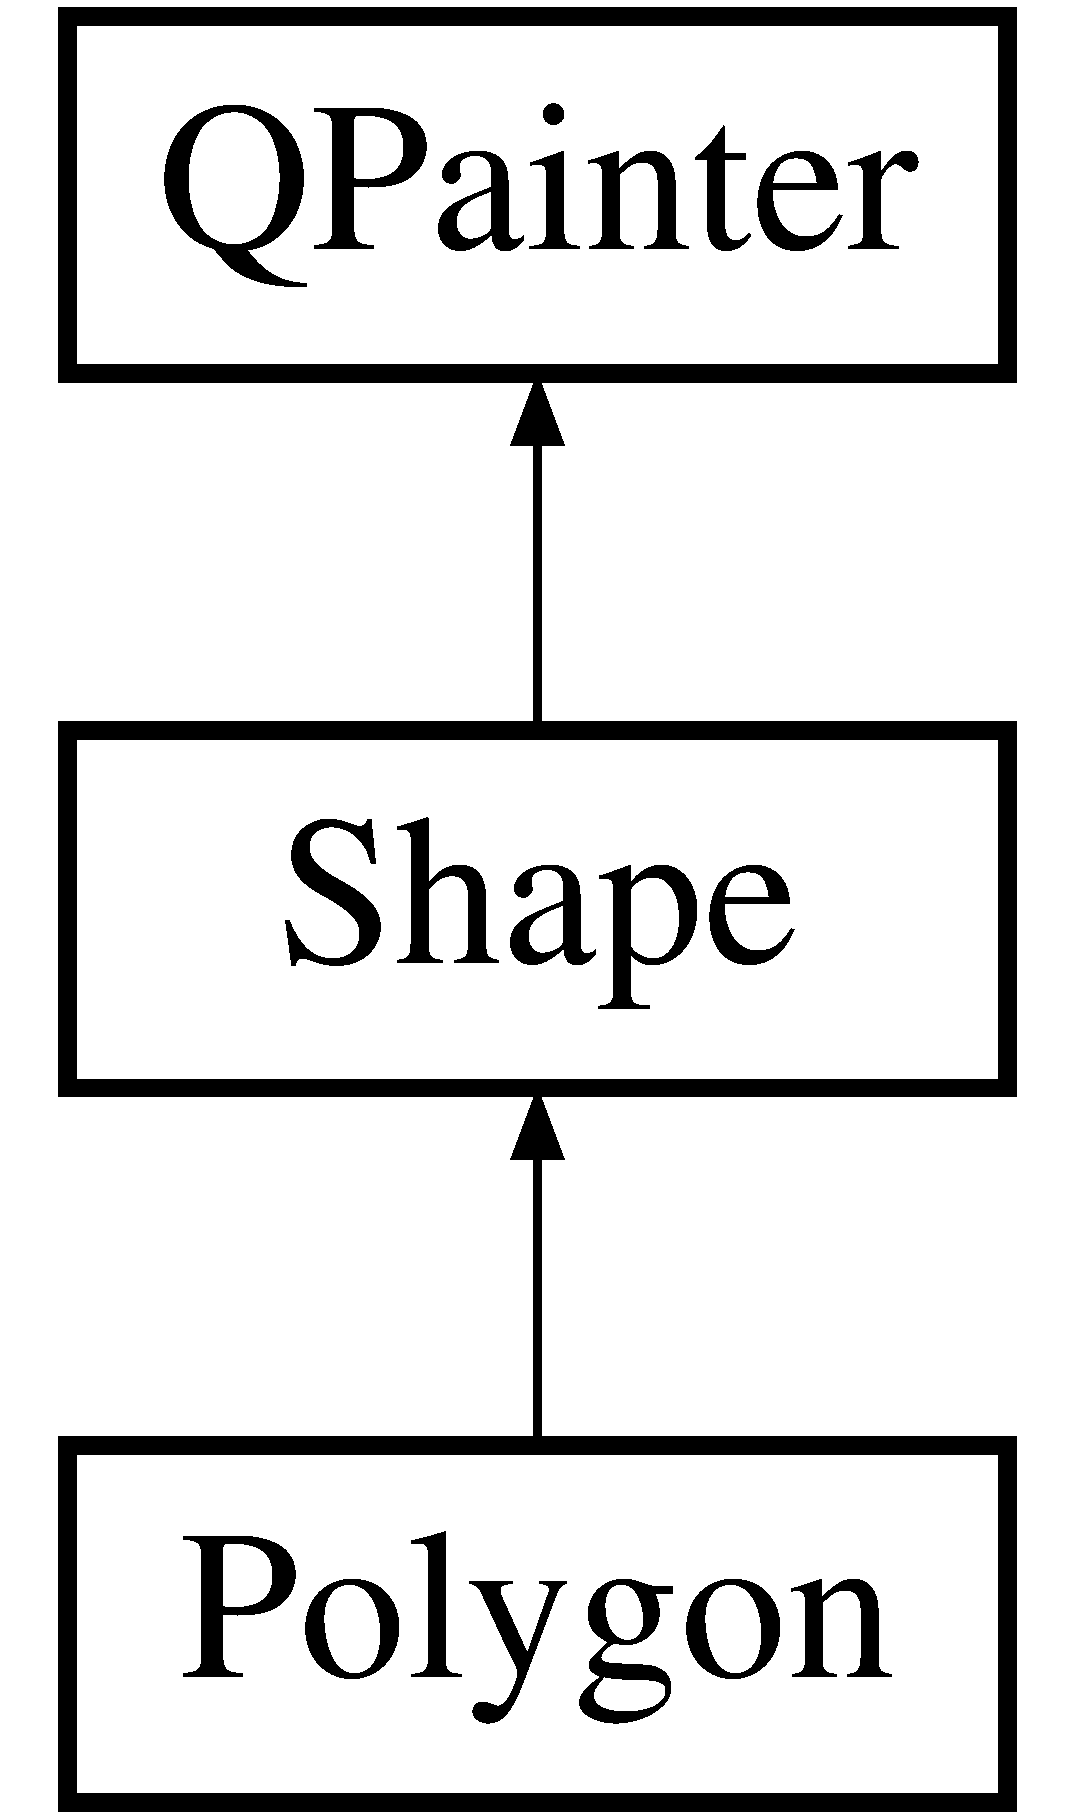
\includegraphics[height=3.000000cm]{class_polygon}
\end{center}
\end{figure}
\subsection*{Public Member Functions}
\begin{DoxyCompactItemize}
\item 
{\bf Polygon} (Q\+Paint\+Device $\ast$dev=nullptr, int id=-\/1)
\begin{DoxyCompactList}\small\item\em \doxyref{Polygon}{p.}{class_polygon} Class constructor. \end{DoxyCompactList}\item 
{\bf $\sim$\+Polygon} () override\label{class_polygon_ad289583dba86760f78296670c95b1eb7}

\begin{DoxyCompactList}\small\item\em \doxyref{Polygon}{p.}{class_polygon} Class Destructor. \end{DoxyCompactList}\item 
virtual void {\bf draw} (Q\+Paint\+Device $\ast$dev) override
\begin{DoxyCompactList}\small\item\em draw function to draw a \doxyref{Polygon}{p.}{class_polygon} \end{DoxyCompactList}\item 
virtual void {\bf move} (int x, int y, int vertex) override
\begin{DoxyCompactList}\small\item\em move function to move a polygon \end{DoxyCompactList}\item 
virtual double {\bf area} () override
\begin{DoxyCompactList}\small\item\em area function to calculate area of polygon \end{DoxyCompactList}\item 
virtual double {\bf perimeter} () override
\begin{DoxyCompactList}\small\item\em perimter function to calculate perimeter of polygon \end{DoxyCompactList}\item 
void {\bf set\+Num\+Vertices} (int num\+Vertices)
\begin{DoxyCompactList}\small\item\em set\+Num\+Vertices function sets the nummber of vertices for the polygon \end{DoxyCompactList}\item 
int {\bf get\+Num\+Vertices} ()
\begin{DoxyCompactList}\small\item\em get\+Num\+Vertices function returns the value of num\+Verts. \end{DoxyCompactList}\item 
void {\bf add\+Vertex} (const Q\+Point \&vertex)
\begin{DoxyCompactList}\small\item\em function to add a vertex to a polygon \end{DoxyCompactList}\item 
Awesome\+Vector$<$ Q\+Point $>$ \& {\bf get\+Vertices} ()\label{class_polygon_ae64510c2f326153369493ac560639b43}

\begin{DoxyCompactList}\small\item\em function to return points to make shapes. \end{DoxyCompactList}\end{DoxyCompactItemize}
\subsection*{Additional Inherited Members}


\subsection{Detailed Description}
\doxyref{Polygon}{p.}{class_polygon} Class\+: Public Inheritance from \doxyref{Shape}{p.}{class_shape} Class. 

\subsection{Constructor \& Destructor Documentation}
\index{Polygon@{Polygon}!Polygon@{Polygon}}
\index{Polygon@{Polygon}!Polygon@{Polygon}}
\subsubsection[{Polygon(\+Q\+Paint\+Device $\ast$dev=nullptr, int id=-\/1)}]{\setlength{\rightskip}{0pt plus 5cm}Polygon\+::\+Polygon (
\begin{DoxyParamCaption}
\item[{Q\+Paint\+Device $\ast$}]{dev = {\ttfamily nullptr}, }
\item[{int}]{id = {\ttfamily -\/1}}
\end{DoxyParamCaption}
)}\label{class_polygon_acbbfa318bb3450651c7bfdd9848df1d1}


\doxyref{Polygon}{p.}{class_polygon} Class constructor. 


\begin{DoxyParams}{Parameters}
{\em $\ast$dev} & is a pointer of type Q\+Paint\+Device, intialized to nullptr to avoid conflicts \\
\hline
{\em id} & is of type int \\
\hline
\end{DoxyParams}


\subsection{Member Function Documentation}
\index{Polygon@{Polygon}!add\+Vertex@{add\+Vertex}}
\index{add\+Vertex@{add\+Vertex}!Polygon@{Polygon}}
\subsubsection[{add\+Vertex(const Q\+Point \&vertex)}]{\setlength{\rightskip}{0pt plus 5cm}void Polygon\+::add\+Vertex (
\begin{DoxyParamCaption}
\item[{const Q\+Point \&}]{vertex}
\end{DoxyParamCaption}
)}\label{class_polygon_a38a6c46772caecff4d9462017201209c}


function to add a vertex to a polygon 

add\+Vertex function requires one parameter, no type is returned by the function 
\begin{DoxyParams}{Parameters}
{\em vertex} & is constant reference of type Q\+Point [] \\
\hline
\end{DoxyParams}
\index{Polygon@{Polygon}!area@{area}}
\index{area@{area}!Polygon@{Polygon}}
\subsubsection[{area() override}]{\setlength{\rightskip}{0pt plus 5cm}virtual double Polygon\+::area (
\begin{DoxyParamCaption}
{}
\end{DoxyParamCaption}
)\hspace{0.3cm}{\ttfamily [override]}, {\ttfamily [virtual]}}\label{class_polygon_a648f54300ccf93f6e4f4acf6b96c5ee1}


area function to calculate area of polygon 

area function overrides the virtual area from abstract base class \doxyref{Shape}{p.}{class_shape}. Function returns a double. area function does not take in any parameters. 

Implements {\bf Shape} \doxyref{}{p.}{class_shape_aa3072fde001d5174f78fcc484c11870c}.

\index{Polygon@{Polygon}!draw@{draw}}
\index{draw@{draw}!Polygon@{Polygon}}
\subsubsection[{draw(\+Q\+Paint\+Device $\ast$dev) override}]{\setlength{\rightskip}{0pt plus 5cm}virtual void Polygon\+::draw (
\begin{DoxyParamCaption}
\item[{Q\+Paint\+Device $\ast$}]{dev}
\end{DoxyParamCaption}
)\hspace{0.3cm}{\ttfamily [override]}, {\ttfamily [virtual]}}\label{class_polygon_a245db29f8ae3b480ab4322646bc76610}


draw function to draw a \doxyref{Polygon}{p.}{class_polygon} 

draw function overrides the virtual draw from abstract class \doxyref{Shape}{p.}{class_shape}. Function does not return any type. 
\begin{DoxyParams}{Parameters}
{\em $\ast$dev} & is a pointer of type Q\+Paint\+Device. \\
\hline
\end{DoxyParams}


Implements {\bf Shape} \doxyref{}{p.}{class_shape_ad2ab549a1b0cc0e23af8be1fd1b61a1b}.

\index{Polygon@{Polygon}!get\+Num\+Vertices@{get\+Num\+Vertices}}
\index{get\+Num\+Vertices@{get\+Num\+Vertices}!Polygon@{Polygon}}
\subsubsection[{get\+Num\+Vertices()}]{\setlength{\rightskip}{0pt plus 5cm}int Polygon\+::get\+Num\+Vertices (
\begin{DoxyParamCaption}
{}
\end{DoxyParamCaption}
)}\label{class_polygon_a934ab08f8ac52f0ab522fa668da2c2dc}


get\+Num\+Vertices function returns the value of num\+Verts. 

No Parameters required, return type if of type int \index{Polygon@{Polygon}!move@{move}}
\index{move@{move}!Polygon@{Polygon}}
\subsubsection[{move(int x, int y, int vertex) override}]{\setlength{\rightskip}{0pt plus 5cm}virtual void Polygon\+::move (
\begin{DoxyParamCaption}
\item[{int}]{x, }
\item[{int}]{y, }
\item[{int}]{vertex}
\end{DoxyParamCaption}
)\hspace{0.3cm}{\ttfamily [override]}, {\ttfamily [virtual]}}\label{class_polygon_af322b762481b14fa3e977e59916af77b}


move function to move a polygon 

move function overrides the virtual move from abstract base class \doxyref{Shape}{p.}{class_shape}. Function does not return any type. 
\begin{DoxyParams}{Parameters}
{\em x} & is of type int \\
\hline
{\em y} & is of type int \\
\hline
{\em vertex} & is of type int \\
\hline
\end{DoxyParams}


Implements {\bf Shape} \doxyref{}{p.}{class_shape_a937ef09c5e1c5c640fdef7caf62ba8f2}.

\index{Polygon@{Polygon}!perimeter@{perimeter}}
\index{perimeter@{perimeter}!Polygon@{Polygon}}
\subsubsection[{perimeter() override}]{\setlength{\rightskip}{0pt plus 5cm}virtual double Polygon\+::perimeter (
\begin{DoxyParamCaption}
{}
\end{DoxyParamCaption}
)\hspace{0.3cm}{\ttfamily [override]}, {\ttfamily [virtual]}}\label{class_polygon_a20a7debc31cce7ae94c066d898a46561}


perimter function to calculate perimeter of polygon 

perimeter function overrides the virtual perimeter abstract base class \doxyref{Shape}{p.}{class_shape}. Function returns a double. perimeter function does not take in any parameters. 

Implements {\bf Shape} \doxyref{}{p.}{class_shape_afb064edd78952da66801619338e8c5a3}.

\index{Polygon@{Polygon}!set\+Num\+Vertices@{set\+Num\+Vertices}}
\index{set\+Num\+Vertices@{set\+Num\+Vertices}!Polygon@{Polygon}}
\subsubsection[{set\+Num\+Vertices(int num\+Vertices)}]{\setlength{\rightskip}{0pt plus 5cm}void Polygon\+::set\+Num\+Vertices (
\begin{DoxyParamCaption}
\item[{int}]{num\+Vertices}
\end{DoxyParamCaption}
)}\label{class_polygon_a0ab9c9ec47b65946a9789a38581879ff}


set\+Num\+Vertices function sets the nummber of vertices for the polygon 

The class member variable num\+Verts is set equal to num\+Vertices 
\begin{DoxyParams}{Parameters}
{\em num\+Vertices} & is of type int \\
\hline
\end{DoxyParams}


The documentation for this class was generated from the following file\+:\begin{DoxyCompactItemize}
\item 
Shape.\+h\end{DoxyCompactItemize}

\section{Polyline Class Reference}
\label{class_polyline}\index{Polyline@{Polyline}}


\doxyref{Polyline}{p.}{class_polyline} Class\+: Public Inheritance from \doxyref{Shape}{p.}{class_shape} Class.  




{\ttfamily \#include $<$Shape.\+h$>$}

Inheritance diagram for Polyline\+:\begin{figure}[H]
\begin{center}
\leavevmode
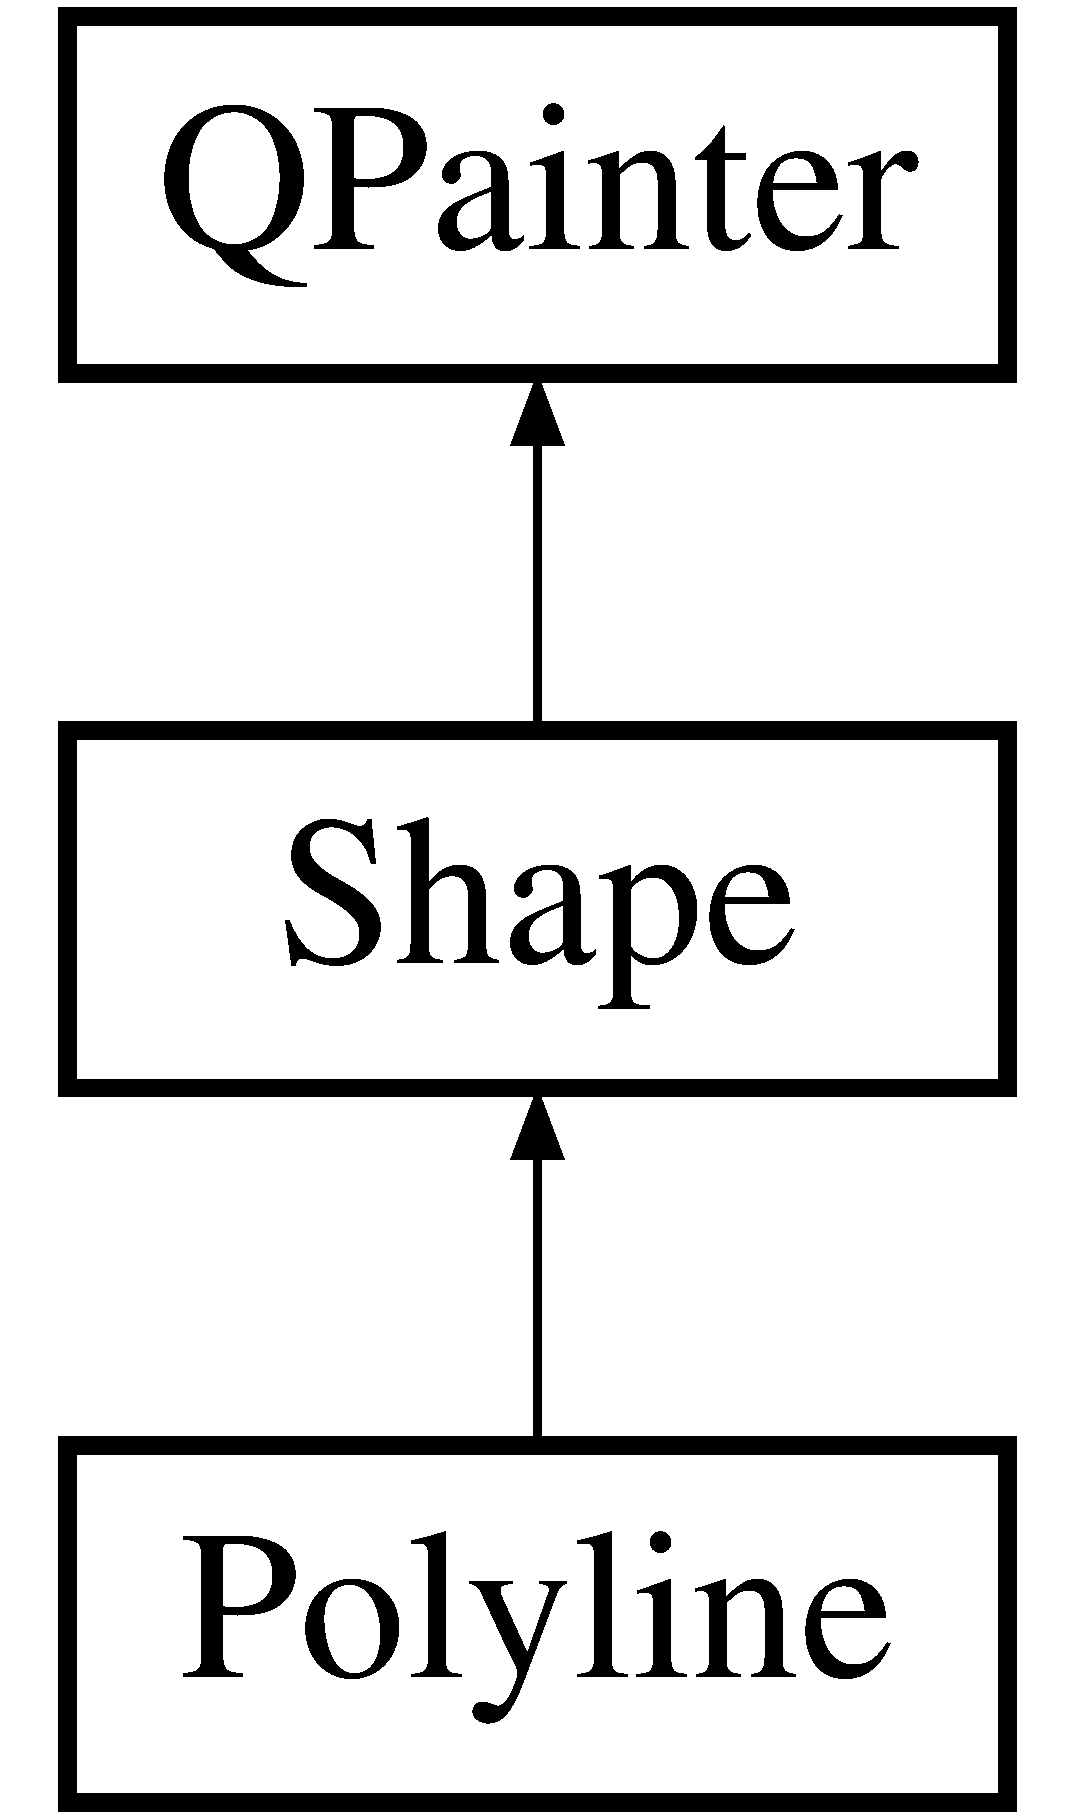
\includegraphics[height=3.000000cm]{class_polyline}
\end{center}
\end{figure}
\subsection*{Public Member Functions}
\begin{DoxyCompactItemize}
\item 
{\bf Polyline} (Q\+Paint\+Device $\ast$device=nullptr, int id=-\/1)
\begin{DoxyCompactList}\small\item\em \doxyref{Polyline}{p.}{class_polyline} Class constructor. \end{DoxyCompactList}\item 
{\bf $\sim$\+Polyline} () override\label{class_polyline_af77a79ed0a14a8334cfd92cd17063fec}

\begin{DoxyCompactList}\small\item\em \doxyref{Polyline}{p.}{class_polyline} Class destructor. \end{DoxyCompactList}\item 
void {\bf add\+Point} (const Q\+Point \&pt)
\begin{DoxyCompactList}\small\item\em add\+Point function to add points to a polyline \end{DoxyCompactList}\item 
void {\bf add\+Num\+Points} (int num)
\begin{DoxyCompactList}\small\item\em add\+Num\+Points function to set class member variable num\+Pts, takes in an int \end{DoxyCompactList}\item 
virtual void {\bf draw} (Q\+Paint\+Device $\ast$device) override
\begin{DoxyCompactList}\small\item\em draw function to draw a polyline \end{DoxyCompactList}\item 
void {\bf move} (int x, int y, int vertex) override
\begin{DoxyCompactList}\small\item\em move function to move a polyline \end{DoxyCompactList}\item 
double {\bf perimeter} () override
\begin{DoxyCompactList}\small\item\em perimeter function to calculate perimeter of a polyline \end{DoxyCompactList}\item 
double {\bf area} () override
\begin{DoxyCompactList}\small\item\em area function to calculate area of a polyline \end{DoxyCompactList}\item 
Awesome\+Vector$<$ Q\+Point $>$ \& {\bf get\+Points} ()\label{class_polyline_a4583e6c29cb39db29fdae796f7968632}

\begin{DoxyCompactList}\small\item\em function to return points to make shapes. \end{DoxyCompactList}\item 
int {\bf get\+Num\+Points} ()\label{class_polyline_a80b8c56a38d4dcf70ac9f3bd314aec2b}

\begin{DoxyCompactList}\small\item\em get\+Num\+Points returns the number of points within polyline \end{DoxyCompactList}\end{DoxyCompactItemize}
\subsection*{Additional Inherited Members}


\subsection{Detailed Description}
\doxyref{Polyline}{p.}{class_polyline} Class\+: Public Inheritance from \doxyref{Shape}{p.}{class_shape} Class. 

\subsection{Constructor \& Destructor Documentation}
\index{Polyline@{Polyline}!Polyline@{Polyline}}
\index{Polyline@{Polyline}!Polyline@{Polyline}}
\subsubsection[{Polyline(\+Q\+Paint\+Device $\ast$device=nullptr, int id=-\/1)}]{\setlength{\rightskip}{0pt plus 5cm}Polyline\+::\+Polyline (
\begin{DoxyParamCaption}
\item[{Q\+Paint\+Device $\ast$}]{device = {\ttfamily nullptr}, }
\item[{int}]{id = {\ttfamily -\/1}}
\end{DoxyParamCaption}
)}\label{class_polyline_a2587221692617dcbd2d8cf4e82d1857a}


\doxyref{Polyline}{p.}{class_polyline} Class constructor. 

\doxyref{Polyline}{p.}{class_polyline} Class constructor takes in two arguments 
\begin{DoxyParams}{Parameters}
{\em $\ast$device} & is a pointer of type Q\+Paint\+Device, initialized to nullptr to avoid conflict \\
\hline
{\em id} & is of type int \\
\hline
\end{DoxyParams}


\subsection{Member Function Documentation}
\index{Polyline@{Polyline}!add\+Num\+Points@{add\+Num\+Points}}
\index{add\+Num\+Points@{add\+Num\+Points}!Polyline@{Polyline}}
\subsubsection[{add\+Num\+Points(int num)}]{\setlength{\rightskip}{0pt plus 5cm}void Polyline\+::add\+Num\+Points (
\begin{DoxyParamCaption}
\item[{int}]{num}
\end{DoxyParamCaption}
)\hspace{0.3cm}{\ttfamily [inline]}}\label{class_polyline_a947a2b96443f0759b047b27a805903c4}


add\+Num\+Points function to set class member variable num\+Pts, takes in an int 


\begin{DoxyParams}{Parameters}
{\em is} & an int \\
\hline
\end{DoxyParams}
\index{Polyline@{Polyline}!add\+Point@{add\+Point}}
\index{add\+Point@{add\+Point}!Polyline@{Polyline}}
\subsubsection[{add\+Point(const Q\+Point \&pt)}]{\setlength{\rightskip}{0pt plus 5cm}void Polyline\+::add\+Point (
\begin{DoxyParamCaption}
\item[{const Q\+Point \&}]{pt}
\end{DoxyParamCaption}
)}\label{class_polyline_a0f72a85f41fcdbcf32f9029e7c717ff3}


add\+Point function to add points to a polyline 

add\+Point takes in at most one argument 
\begin{DoxyParams}{Parameters}
{\em pt} & is a constant reference of type Q\+Point \\
\hline
\end{DoxyParams}
\index{Polyline@{Polyline}!area@{area}}
\index{area@{area}!Polyline@{Polyline}}
\subsubsection[{area() override}]{\setlength{\rightskip}{0pt plus 5cm}double Polyline\+::area (
\begin{DoxyParamCaption}
{}
\end{DoxyParamCaption}
)\hspace{0.3cm}{\ttfamily [inline]}, {\ttfamily [override]}, {\ttfamily [virtual]}}\label{class_polyline_a94f6c78fc78eaf2efd0d5221fd7b44dc}


area function to calculate area of a polyline 

area function overrides the virtual area function of abstract base class shape. Function returns a double. No parameters are passed into area, polyline does not have area so the function is defined only by \char`\"{}return 0\char`\"{}. Function definition must be defined as return 0, else line class will be recognized as an abstract class. 

Implements {\bf Shape} \doxyref{}{p.}{class_shape_aa3072fde001d5174f78fcc484c11870c}.

\index{Polyline@{Polyline}!draw@{draw}}
\index{draw@{draw}!Polyline@{Polyline}}
\subsubsection[{draw(\+Q\+Paint\+Device $\ast$device) override}]{\setlength{\rightskip}{0pt plus 5cm}virtual void Polyline\+::draw (
\begin{DoxyParamCaption}
\item[{Q\+Paint\+Device $\ast$}]{device}
\end{DoxyParamCaption}
)\hspace{0.3cm}{\ttfamily [override]}, {\ttfamily [virtual]}}\label{class_polyline_a852420931a45f831deaff590c40b150c}


draw function to draw a polyline 

draw function overrides the virtual draw from abstract base class shape. Funtion does not return any type. 
\begin{DoxyParams}{Parameters}
{\em $\ast$device} & is a pointer of type Q\+Paint\+Device \\
\hline
\end{DoxyParams}


Implements {\bf Shape} \doxyref{}{p.}{class_shape_ad2ab549a1b0cc0e23af8be1fd1b61a1b}.

\index{Polyline@{Polyline}!move@{move}}
\index{move@{move}!Polyline@{Polyline}}
\subsubsection[{move(int x, int y, int vertex) override}]{\setlength{\rightskip}{0pt plus 5cm}void Polyline\+::move (
\begin{DoxyParamCaption}
\item[{int}]{x, }
\item[{int}]{y, }
\item[{int}]{vertex}
\end{DoxyParamCaption}
)\hspace{0.3cm}{\ttfamily [override]}, {\ttfamily [virtual]}}\label{class_polyline_a33cd81f76e084f77ffcd9304c879354e}


move function to move a polyline 

move function overrides the virtual move from abstract base class \doxyref{Shape}{p.}{class_shape}. Function does not return any type. 
\begin{DoxyParams}{Parameters}
{\em x} & is of type int \\
\hline
{\em y} & is of type int \\
\hline
{\em vertex} & is of type int \\
\hline
\end{DoxyParams}


Implements {\bf Shape} \doxyref{}{p.}{class_shape_a937ef09c5e1c5c640fdef7caf62ba8f2}.

\index{Polyline@{Polyline}!perimeter@{perimeter}}
\index{perimeter@{perimeter}!Polyline@{Polyline}}
\subsubsection[{perimeter() override}]{\setlength{\rightskip}{0pt plus 5cm}double Polyline\+::perimeter (
\begin{DoxyParamCaption}
{}
\end{DoxyParamCaption}
)\hspace{0.3cm}{\ttfamily [inline]}, {\ttfamily [override]}, {\ttfamily [virtual]}}\label{class_polyline_a1c9bb62b882f1c97d6aaa40755dc8746}


perimeter function to calculate perimeter of a polyline 

perimeter function overrides the virtual perimeter function of abstract base class shape. Function returns a double. No parameters are passed into perimeter, polyline does not have perimeter so the function is defined only by \char`\"{}return 0\char`\"{}. Function definition must be defined as return 0, else line class will be recognized as an abstract class. 

Implements {\bf Shape} \doxyref{}{p.}{class_shape_afb064edd78952da66801619338e8c5a3}.



The documentation for this class was generated from the following file\+:\begin{DoxyCompactItemize}
\item 
Shape.\+h\end{DoxyCompactItemize}

\section{Rectangle Class Reference}
\label{class_rectangle}\index{Rectangle@{Rectangle}}


\doxyref{Rectangle}{p.}{class_rectangle} Class\+: Public Inheritance from \doxyref{Shape}{p.}{class_shape} Class.  




{\ttfamily \#include $<$Shape.\+h$>$}

Inheritance diagram for Rectangle\+:\begin{figure}[H]
\begin{center}
\leavevmode
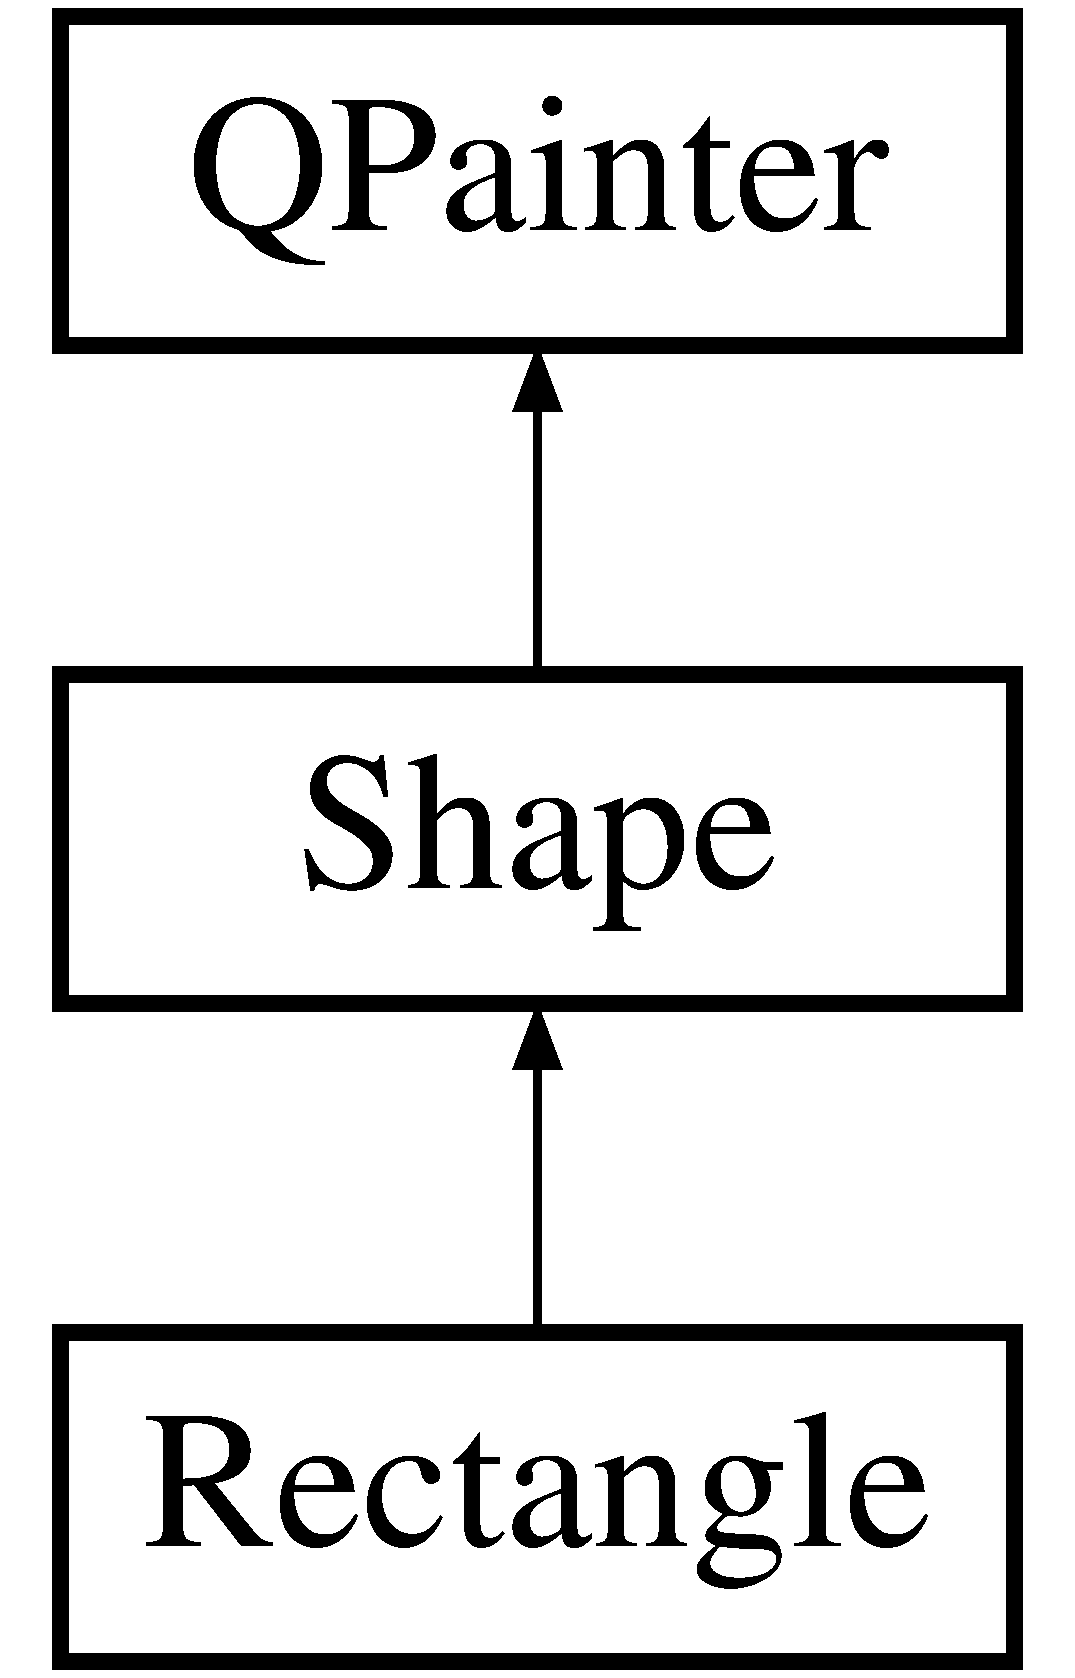
\includegraphics[height=3.000000cm]{class_rectangle}
\end{center}
\end{figure}
\subsection*{Public Member Functions}
\begin{DoxyCompactItemize}
\item 
{\bf Rectangle} (Q\+Paint\+Device $\ast$device=nullptr, int id=-\/1)
\begin{DoxyCompactList}\small\item\em \doxyref{Rectangle}{p.}{class_rectangle} Class Constructor. \end{DoxyCompactList}\item 
{\bf $\sim$\+Rectangle} () override\label{class_rectangle_a6e3ed18583022b35e04c109345d1e7d6}

\begin{DoxyCompactList}\small\item\em \doxyref{Rectangle}{p.}{class_rectangle} Class Destructor. \end{DoxyCompactList}\item 
void {\bf draw} (Q\+Paint\+Device $\ast$device) override
\begin{DoxyCompactList}\small\item\em draw function to draw a rectangle \end{DoxyCompactList}\item 
void {\bf move} (int x, int y, int junk) override
\begin{DoxyCompactList}\small\item\em move function to move a rectangle \end{DoxyCompactList}\item 
double {\bf area} () override
\begin{DoxyCompactList}\small\item\em area function to calculate area of rectangle \end{DoxyCompactList}\item 
double {\bf perimeter} () override
\begin{DoxyCompactList}\small\item\em perimeter function to calculate perimeter of rectangle \end{DoxyCompactList}\item 
void {\bf set\+Location} (int x, int y)
\begin{DoxyCompactList}\small\item\em set\+Location function for rectangle \end{DoxyCompactList}\item 
void {\bf set\+Location} (Q\+Point pt)
\begin{DoxyCompactList}\small\item\em set\+Location function for rectangle \end{DoxyCompactList}\item 
void {\bf set\+Dimensions} (double w, double h)
\begin{DoxyCompactList}\small\item\em set\+Dimensions function for rectangle \end{DoxyCompactList}\item 
void {\bf set\+All} (double w, double h, int x, int y)
\item 
double {\bf get\+Width} ()\label{class_rectangle_a9911b718370d9f9c987c1c5f85379b09}

\begin{DoxyCompactList}\small\item\em get\+Width function for rectangle class, function returns a double width \end{DoxyCompactList}\item 
double {\bf get\+Height} ()\label{class_rectangle_a78c23ebff32769d54b568536d76af7f8}

\begin{DoxyCompactList}\small\item\em get\+Height function for rectangle class, function returns a double height \end{DoxyCompactList}\item 
Q\+Point \& {\bf get\+Location} ()\label{class_rectangle_ad8582dd6add9118e20ab354d6f87bc91}

\begin{DoxyCompactList}\small\item\em get\+Location function for rectangle class, function returns a Q\+Point location \end{DoxyCompactList}\end{DoxyCompactItemize}
\subsection*{Additional Inherited Members}


\subsection{Detailed Description}
\doxyref{Rectangle}{p.}{class_rectangle} Class\+: Public Inheritance from \doxyref{Shape}{p.}{class_shape} Class. 

\subsection{Constructor \& Destructor Documentation}
\index{Rectangle@{Rectangle}!Rectangle@{Rectangle}}
\index{Rectangle@{Rectangle}!Rectangle@{Rectangle}}
\subsubsection[{Rectangle(\+Q\+Paint\+Device $\ast$device=nullptr, int id=-\/1)}]{\setlength{\rightskip}{0pt plus 5cm}Rectangle\+::\+Rectangle (
\begin{DoxyParamCaption}
\item[{Q\+Paint\+Device $\ast$}]{device = {\ttfamily nullptr}, }
\item[{int}]{id = {\ttfamily -\/1}}
\end{DoxyParamCaption}
)}\label{class_rectangle_a0deed87f87e92f3b48621ff91d7e544f}


\doxyref{Rectangle}{p.}{class_rectangle} Class Constructor. 

\doxyref{Rectangle}{p.}{class_rectangle} Class constructor takes in two arguments. 
\begin{DoxyParams}{Parameters}
{\em $\ast$device} & is a pointer of type Q\+Paint\+Device, initialized to nullptr to avoid conflict \\
\hline
{\em id} & is of type int \\
\hline
\end{DoxyParams}


\subsection{Member Function Documentation}
\index{Rectangle@{Rectangle}!area@{area}}
\index{area@{area}!Rectangle@{Rectangle}}
\subsubsection[{area() override}]{\setlength{\rightskip}{0pt plus 5cm}double Rectangle\+::area (
\begin{DoxyParamCaption}
{}
\end{DoxyParamCaption}
)\hspace{0.3cm}{\ttfamily [override]}, {\ttfamily [virtual]}}\label{class_rectangle_a6b3912c47937ed46693249ad0b8081c9}


area function to calculate area of rectangle 

area function overrides the virtual area function of abstract base class shape. Function returns a double. No parameters are passed into area. 

Implements {\bf Shape} \doxyref{}{p.}{class_shape_aa3072fde001d5174f78fcc484c11870c}.

\index{Rectangle@{Rectangle}!draw@{draw}}
\index{draw@{draw}!Rectangle@{Rectangle}}
\subsubsection[{draw(\+Q\+Paint\+Device $\ast$device) override}]{\setlength{\rightskip}{0pt plus 5cm}void Rectangle\+::draw (
\begin{DoxyParamCaption}
\item[{Q\+Paint\+Device $\ast$}]{device}
\end{DoxyParamCaption}
)\hspace{0.3cm}{\ttfamily [override]}, {\ttfamily [virtual]}}\label{class_rectangle_aa7b84289ee0e504fd5dee6fe5aa7f425}


draw function to draw a rectangle 

draw function overrides the virtual draw from abstract base class shape. Funtion does not return any type. 
\begin{DoxyParams}{Parameters}
{\em $\ast$device} & is a pointer of type Q\+Paint\+Device \\
\hline
\end{DoxyParams}


Implements {\bf Shape} \doxyref{}{p.}{class_shape_ad2ab549a1b0cc0e23af8be1fd1b61a1b}.

\index{Rectangle@{Rectangle}!move@{move}}
\index{move@{move}!Rectangle@{Rectangle}}
\subsubsection[{move(int x, int y, int junk) override}]{\setlength{\rightskip}{0pt plus 5cm}void Rectangle\+::move (
\begin{DoxyParamCaption}
\item[{int}]{x, }
\item[{int}]{y, }
\item[{int}]{junk}
\end{DoxyParamCaption}
)\hspace{0.3cm}{\ttfamily [override]}, {\ttfamily [virtual]}}\label{class_rectangle_a6f689d4bcf53f18bd4325200259a9da3}


move function to move a rectangle 

move function overrides the virtual move from abstract base class \doxyref{Shape}{p.}{class_shape}. Function does not return any type. 
\begin{DoxyParams}{Parameters}
{\em x} & is of type int \\
\hline
{\em y} & is of type int \\
\hline
{\em junk} & is of type int \\
\hline
\end{DoxyParams}


Implements {\bf Shape} \doxyref{}{p.}{class_shape_a937ef09c5e1c5c640fdef7caf62ba8f2}.

\index{Rectangle@{Rectangle}!perimeter@{perimeter}}
\index{perimeter@{perimeter}!Rectangle@{Rectangle}}
\subsubsection[{perimeter() override}]{\setlength{\rightskip}{0pt plus 5cm}double Rectangle\+::perimeter (
\begin{DoxyParamCaption}
{}
\end{DoxyParamCaption}
)\hspace{0.3cm}{\ttfamily [override]}, {\ttfamily [virtual]}}\label{class_rectangle_a1672f74c28fa25703683f13d02e182a6}


perimeter function to calculate perimeter of rectangle 

perimeter function overrides the virtual perimeter function of abstract base class shape. Function returns a double. No parameters are passed into perimeter. 

Implements {\bf Shape} \doxyref{}{p.}{class_shape_afb064edd78952da66801619338e8c5a3}.

\index{Rectangle@{Rectangle}!set\+All@{set\+All}}
\index{set\+All@{set\+All}!Rectangle@{Rectangle}}
\subsubsection[{set\+All(double w, double h, int x, int y)}]{\setlength{\rightskip}{0pt plus 5cm}void Rectangle\+::set\+All (
\begin{DoxyParamCaption}
\item[{double}]{w, }
\item[{double}]{h, }
\item[{int}]{x, }
\item[{int}]{y}
\end{DoxyParamCaption}
)}\label{class_rectangle_a583a73ee34b4ce7b60459922dbb2094d}
set\+All function requires four parameters. The class member functions width, height, location are set from these arguments. In this function, the set\+Location and set\+Dimension functions are being called. 
\begin{DoxyParams}{Parameters}
{\em w} & is of type double \\
\hline
{\em h} & is of type double \\
\hline
{\em x} & is of type int \\
\hline
{\em y} & is of type int \\
\hline
\end{DoxyParams}
\index{Rectangle@{Rectangle}!set\+Dimensions@{set\+Dimensions}}
\index{set\+Dimensions@{set\+Dimensions}!Rectangle@{Rectangle}}
\subsubsection[{set\+Dimensions(double w, double h)}]{\setlength{\rightskip}{0pt plus 5cm}void Rectangle\+::set\+Dimensions (
\begin{DoxyParamCaption}
\item[{double}]{w, }
\item[{double}]{h}
\end{DoxyParamCaption}
)}\label{class_rectangle_a10a5a88119f55914c1d9d68a7678d457}


set\+Dimensions function for rectangle 

set\+Dimensions function requires two parameters. The class member variables width and height are set from these parameters. 
\begin{DoxyParams}{Parameters}
{\em w} & is of type double \\
\hline
{\em h} & is of type double \\
\hline
\end{DoxyParams}
\index{Rectangle@{Rectangle}!set\+Location@{set\+Location}}
\index{set\+Location@{set\+Location}!Rectangle@{Rectangle}}
\subsubsection[{set\+Location(int x, int y)}]{\setlength{\rightskip}{0pt plus 5cm}void Rectangle\+::set\+Location (
\begin{DoxyParamCaption}
\item[{int}]{x, }
\item[{int}]{y}
\end{DoxyParamCaption}
)}\label{class_rectangle_a6d2dd7280e01d1d3a044a852d0b42619}


set\+Location function for rectangle 

set\+Location function requires two arguments. Takes the two arguments and makes a coordinate pair (Q\+Point) consisting of these values. 
\begin{DoxyParams}{Parameters}
{\em x} & is of type int \\
\hline
{\em y} & is of type int \\
\hline
\end{DoxyParams}
\index{Rectangle@{Rectangle}!set\+Location@{set\+Location}}
\index{set\+Location@{set\+Location}!Rectangle@{Rectangle}}
\subsubsection[{set\+Location(\+Q\+Point pt)}]{\setlength{\rightskip}{0pt plus 5cm}void Rectangle\+::set\+Location (
\begin{DoxyParamCaption}
\item[{Q\+Point}]{pt}
\end{DoxyParamCaption}
)}\label{class_rectangle_a3e38c916a6685543e8a2196f25d6ebdc}


set\+Location function for rectangle 

set\+Location function requires a single parameter. The class memeber variable location is set to the Q\+Point parameter passed in. 
\begin{DoxyParams}{Parameters}
{\em pt} & is of type Q\+Point \\
\hline
\end{DoxyParams}


The documentation for this class was generated from the following file\+:\begin{DoxyCompactItemize}
\item 
Shape.\+h\end{DoxyCompactItemize}

\section{Render\+Area Class Reference}
\label{class_render_area}\index{Render\+Area@{Render\+Area}}


\doxyref{Render\+Area}{p.}{class_render_area} Class\+: Public Inheritance from Q\+Widget.  




{\ttfamily \#include $<$Render\+Area.\+h$>$}

Inheritance diagram for Render\+Area\+:\begin{figure}[H]
\begin{center}
\leavevmode
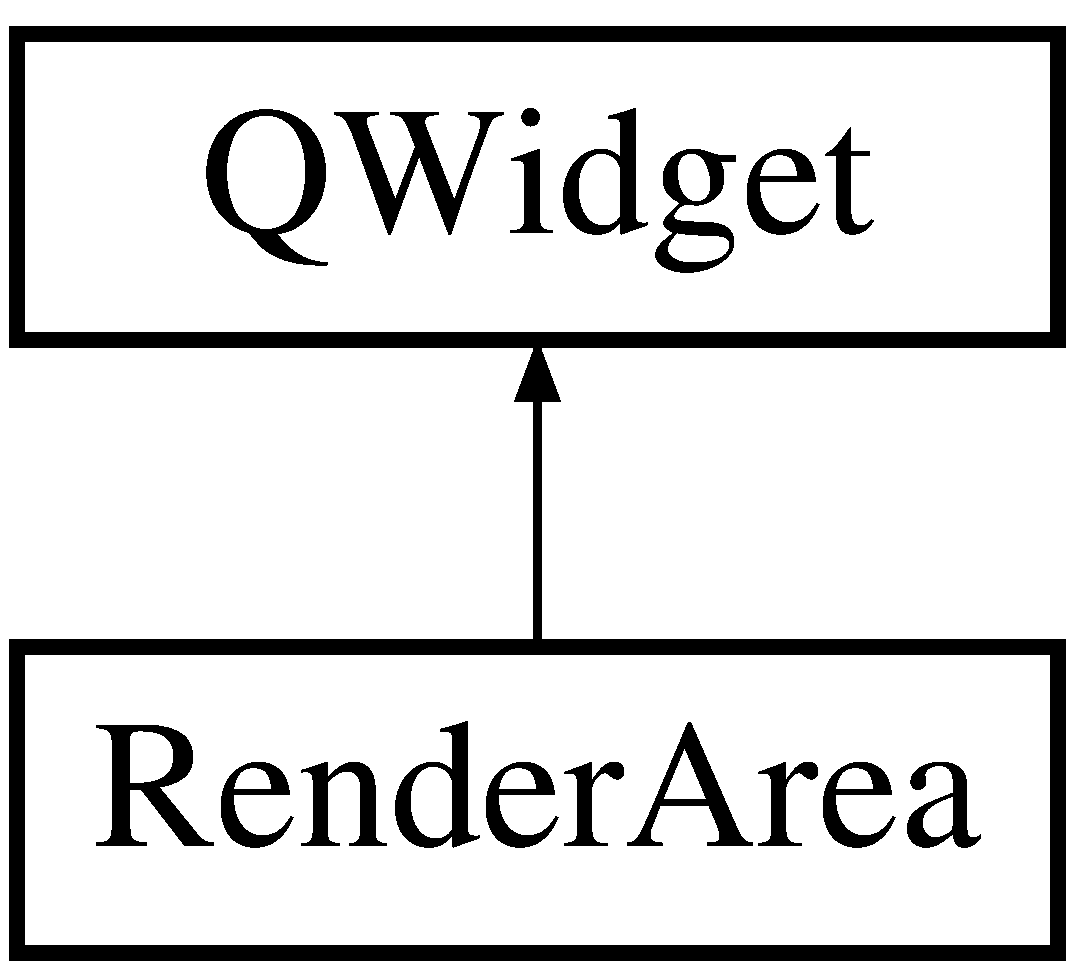
\includegraphics[height=2.000000cm]{class_render_area}
\end{center}
\end{figure}
\subsection*{Public Member Functions}
\begin{DoxyCompactItemize}
\item 
{\bf Render\+Area} (Q\+Widget $\ast$parent=nullptr)
\begin{DoxyCompactList}\small\item\em \doxyref{Render\+Area}{p.}{class_render_area} Class Constutor. \end{DoxyCompactList}\item 
void {\bf paint\+Event} (Q\+Paint\+Event $\ast$event) override
\begin{DoxyCompactList}\small\item\em paint\+Event function for \doxyref{Render\+Area}{p.}{class_render_area} \end{DoxyCompactList}\item 
Q\+Size {\bf size\+Hint} () const override
\begin{DoxyCompactList}\small\item\em size\+Hint function for \doxyref{Render\+Area}{p.}{class_render_area} \end{DoxyCompactList}\item 
Q\+Size {\bf minimum\+Size\+Hint} () const override
\begin{DoxyCompactList}\small\item\em minimum\+Size\+Hint function for \doxyref{Render\+Area}{p.}{class_render_area} \end{DoxyCompactList}\item 
const Awesome\+Vector$<$ {\bf Shape} $\ast$ $>$ \& {\bfseries get\+Shapes} ()\label{class_render_area_a02724ed9e0a5a14f845715be591bc9a5}

\item 
void {\bf add\+Shape} ({\bf Shape} $\ast$shape\+In)
\begin{DoxyCompactList}\small\item\em add\+Shape function for \doxyref{Render\+Area}{p.}{class_render_area} \end{DoxyCompactList}\item 
int {\bf get\+Size} ()
\begin{DoxyCompactList}\small\item\em get\+Size function for \doxyref{Render\+Area}{p.}{class_render_area} \end{DoxyCompactList}\item 
int {\bf get\+Num\+Shapes} ()\label{class_render_area_ab83495add26bd1613960ec46a49f9ea6}

\begin{DoxyCompactList}\small\item\em get\+Num\+Shapes function for \doxyref{Render\+Area}{p.}{class_render_area} \end{DoxyCompactList}\item 
void {\bf chop\+Shape} (int index\+Remove)\label{class_render_area_ab5846cdc9daaa9f83e7b4de78ba33be0}

\begin{DoxyCompactList}\small\item\em chop\+Shape function for \doxyref{Render\+Area}{p.}{class_render_area} \end{DoxyCompactList}\item 
void {\bf move\+Shape} (int index\+Move, int coord\+Move, int x, int y)
\begin{DoxyCompactList}\small\item\em move\+Shape fucntion for \doxyref{Render\+Area}{p.}{class_render_area} \end{DoxyCompactList}\end{DoxyCompactItemize}


\subsection{Detailed Description}
\doxyref{Render\+Area}{p.}{class_render_area} Class\+: Public Inheritance from Q\+Widget. 

\doxyref{Render\+Area}{p.}{class_render_area} is inheriting from Q\+Widget, thus has all the functionalities of Q\+Widget plus additional functions and variables that allow rendering of shapes defined by the shape class heirarchy. 

\subsection{Constructor \& Destructor Documentation}
\index{Render\+Area@{Render\+Area}!Render\+Area@{Render\+Area}}
\index{Render\+Area@{Render\+Area}!Render\+Area@{Render\+Area}}
\subsubsection[{Render\+Area(\+Q\+Widget $\ast$parent=nullptr)}]{\setlength{\rightskip}{0pt plus 5cm}Render\+Area\+::\+Render\+Area (
\begin{DoxyParamCaption}
\item[{Q\+Widget $\ast$}]{parent = {\ttfamily nullptr}}
\end{DoxyParamCaption}
)}\label{class_render_area_a6fa5a406003dc132605f8bc07763e946}


\doxyref{Render\+Area}{p.}{class_render_area} Class Constutor. 

\doxyref{Render\+Area}{p.}{class_render_area} Constructor takes in one paramater of type Q\+Widget$\ast$, initilaized to nullptr to avoid conflict. Q\+Widget is the base class for all user-\/interface objects 
\begin{DoxyParams}{Parameters}
{\em $\ast$parent} & is of type Q\+Widget \\
\hline
\end{DoxyParams}


\subsection{Member Function Documentation}
\index{Render\+Area@{Render\+Area}!add\+Shape@{add\+Shape}}
\index{add\+Shape@{add\+Shape}!Render\+Area@{Render\+Area}}
\subsubsection[{add\+Shape(\+Shape $\ast$shape\+In)}]{\setlength{\rightskip}{0pt plus 5cm}void Render\+Area\+::add\+Shape (
\begin{DoxyParamCaption}
\item[{{\bf Shape} $\ast$}]{shape\+In}
\end{DoxyParamCaption}
)}\label{class_render_area_a7267206d6c6eeef44766fd4f2fd66046}


add\+Shape function for \doxyref{Render\+Area}{p.}{class_render_area} 

add\+Shape adds a shape to the end of the class vector Shape\+Magazine. add\+Shape requires one parameter 
\begin{DoxyParams}{Parameters}
{\em shape\+In$\ast$} & is a pointer of type \doxyref{Shape}{p.}{class_shape}, nothing is being returned \\
\hline
\end{DoxyParams}
\index{Render\+Area@{Render\+Area}!get\+Size@{get\+Size}}
\index{get\+Size@{get\+Size}!Render\+Area@{Render\+Area}}
\subsubsection[{get\+Size()}]{\setlength{\rightskip}{0pt plus 5cm}int Render\+Area\+::get\+Size (
\begin{DoxyParamCaption}
{}
\end{DoxyParamCaption}
)}\label{class_render_area_a7d8692300a83a722094ff6ed5f29b627}


get\+Size function for \doxyref{Render\+Area}{p.}{class_render_area} 

get\+Size returns the current size of the vector Shape\+Magazine. No parameters are required, and int value is returned \index{Render\+Area@{Render\+Area}!minimum\+Size\+Hint@{minimum\+Size\+Hint}}
\index{minimum\+Size\+Hint@{minimum\+Size\+Hint}!Render\+Area@{Render\+Area}}
\subsubsection[{minimum\+Size\+Hint() const override}]{\setlength{\rightskip}{0pt plus 5cm}Q\+Size Render\+Area\+::minimum\+Size\+Hint (
\begin{DoxyParamCaption}
{}
\end{DoxyParamCaption}
) const\hspace{0.3cm}{\ttfamily [override]}}\label{class_render_area_a323aaf2ce457d3a860bcac912ece7473}


minimum\+Size\+Hint function for \doxyref{Render\+Area}{p.}{class_render_area} 

See size\+Hint \index{Render\+Area@{Render\+Area}!move\+Shape@{move\+Shape}}
\index{move\+Shape@{move\+Shape}!Render\+Area@{Render\+Area}}
\subsubsection[{move\+Shape(int index\+Move, int coord\+Move, int x, int y)}]{\setlength{\rightskip}{0pt plus 5cm}void Render\+Area\+::move\+Shape (
\begin{DoxyParamCaption}
\item[{int}]{index\+Move, }
\item[{int}]{coord\+Move, }
\item[{int}]{x, }
\item[{int}]{y}
\end{DoxyParamCaption}
)}\label{class_render_area_abbf372edf98b6ea9952ab79e205ca3a2}


move\+Shape fucntion for \doxyref{Render\+Area}{p.}{class_render_area} 

move\+Shape function finds the shape at the given index and moves it with the given input parameters. Moves the vertices of a given shape. 
\begin{DoxyParams}{Parameters}
{\em index\+Move} & is of type int \\
\hline
{\em coord\+Move} & is of type int \\
\hline
{\em x} & is of type int \\
\hline
{\em y} & is of type int \\
\hline
\end{DoxyParams}
\index{Render\+Area@{Render\+Area}!paint\+Event@{paint\+Event}}
\index{paint\+Event@{paint\+Event}!Render\+Area@{Render\+Area}}
\subsubsection[{paint\+Event(\+Q\+Paint\+Event $\ast$event) override}]{\setlength{\rightskip}{0pt plus 5cm}void Render\+Area\+::paint\+Event (
\begin{DoxyParamCaption}
\item[{Q\+Paint\+Event $\ast$}]{event}
\end{DoxyParamCaption}
)\hspace{0.3cm}{\ttfamily [override]}}\label{class_render_area_ae9b5a1573f3b06590c717c7598ffaae4}


paint\+Event function for \doxyref{Render\+Area}{p.}{class_render_area} 

paint\+Event function overrides a virtual paint\+Event within Q\+Widget, takes in a Q\+Paint\+Event pointer. 
\begin{DoxyParams}{Parameters}
{\em $\ast$event} & is of type Q\+Paint\+Event \\
\hline
\end{DoxyParams}
\index{Render\+Area@{Render\+Area}!size\+Hint@{size\+Hint}}
\index{size\+Hint@{size\+Hint}!Render\+Area@{Render\+Area}}
\subsubsection[{size\+Hint() const override}]{\setlength{\rightskip}{0pt plus 5cm}Q\+Size Render\+Area\+::size\+Hint (
\begin{DoxyParamCaption}
{}
\end{DoxyParamCaption}
) const\hspace{0.3cm}{\ttfamily [override]}}\label{class_render_area_ac0b3e7195c5ba16eaa6590168db0f0cf}


size\+Hint function for \doxyref{Render\+Area}{p.}{class_render_area} 

size\+Hint function sets the size of the 2-\/D \char`\"{}canvas\char`\"{} upon which the shapes will be rendered. size\+Hint uses Q\+Size(int, int) to set the size of the \char`\"{}canvas\char`\"{}. No parameters required. 

The documentation for this class was generated from the following file\+:\begin{DoxyCompactItemize}
\item 
Render\+Area.\+h\end{DoxyCompactItemize}

\section{Shape Class Reference}
\label{class_shape}\index{Shape@{Shape}}


\doxyref{Shape}{p.}{class_shape} Class\+: Public Inheritance from Q\+Painter Class.  




{\ttfamily \#include $<$Shape.\+h$>$}

Inheritance diagram for Shape\+:\begin{figure}[H]
\begin{center}
\leavevmode
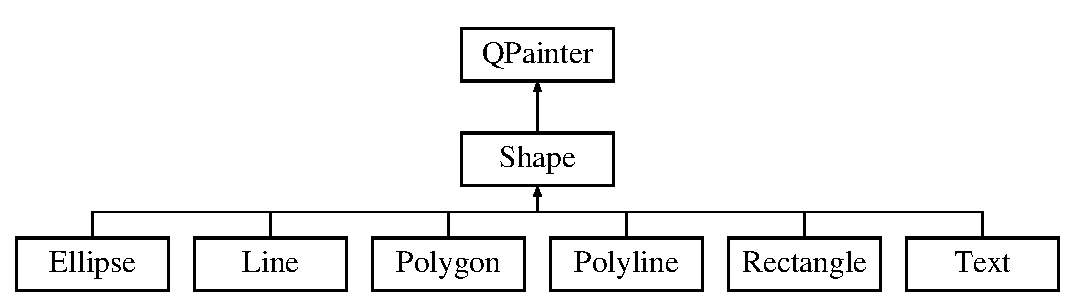
\includegraphics[height=3.000000cm]{class_shape}
\end{center}
\end{figure}
\subsection*{Public Types}
\begin{DoxyCompactItemize}
\item 
enum {\bf Shape\+Type} \{ \\*
{\bfseries null}, 
{\bfseries Line}, 
{\bfseries Polyline}, 
{\bfseries Polygon}, 
\\*
{\bfseries Rectangle}, 
{\bfseries Ellipse}, 
{\bfseries Text}
 \}\begin{DoxyCompactList}\small\item\em Enumeration of Shape\+Type classes. \end{DoxyCompactList}
\end{DoxyCompactItemize}
\subsection*{Public Member Functions}
\begin{DoxyCompactItemize}
\item 
{\bf Shape} (Q\+Paint\+Device $\ast$device=nullptr, int ID=-\/1, {\bf Shape\+Type} shapey=Shape\+Type\+::null)
\begin{DoxyCompactList}\small\item\em \doxyref{Shape}{p.}{class_shape} Class constructor takes in 3 arguments. \end{DoxyCompactList}\item 
virtual {\bf $\sim$\+Shape} ()
\begin{DoxyCompactList}\small\item\em \doxyref{Shape}{p.}{class_shape} Class Destructor. \end{DoxyCompactList}\item 
void {\bf set\+Shape} ({\bf Shape\+Type})
\begin{DoxyCompactList}\small\item\em set\+Shape takes in a Shape\+Type argument \end{DoxyCompactList}\item 
void {\bf set\+Brush} (Qt\+::\+Global\+Color, Qt\+::\+Brush\+Style)
\begin{DoxyCompactList}\small\item\em set\+Brush takes in two Qt type parameters and sets it equal to member variable object shape. \end{DoxyCompactList}\item 
void {\bf set\+Pen} (Qt\+::\+Global\+Color)
\begin{DoxyCompactList}\small\item\em set\+Pen takes in two built-\/in Qt namespaces. \end{DoxyCompactList}\item 
void {\bf set\+Pen} (Qt\+::\+Global\+Color, int width, Qt\+::\+Pen\+Style, Qt\+::\+Pen\+Cap\+Style, Qt\+::\+Pen\+Join\+Style)
\begin{DoxyCompactList}\small\item\em Alternative set\+Pen sets pen equal to four Qt type parameters and one int parameter. \end{DoxyCompactList}\item 
void {\bf set\+Brush} (Q\+Brush brsh)\label{class_shape_a9902d301bf27dae6ffc4a81ff566bfa3}

\begin{DoxyCompactList}\small\item\em set\+Brush takes in a Q\+Brush variable and sets brush to brsh \end{DoxyCompactList}\item 
void {\bf set\+Pen} (Q\+Pen pn)\label{class_shape_a3cabd869e27b2662bf75b980d1795f32}

\begin{DoxyCompactList}\small\item\em set\+Pen takes in a Q\+Pen variable and sets pen to pn \end{DoxyCompactList}\item 
void {\bf set\+ID} (int ID)\label{class_shape_ab5f7a5775837a4c4d4187d901990c1c2}

\begin{DoxyCompactList}\small\item\em set\+ID takes in a int ID and sets id to ID \end{DoxyCompactList}\item 
{\bf Shape\+Type} {\bf get\+Shape} () const \label{class_shape_a0526a3459d426e12f5e754a628bb4bbe}

\begin{DoxyCompactList}\small\item\em get\+Shape returns shape object. \end{DoxyCompactList}\item 
const Q\+Brush \& {\bf get\+Brush} () const \label{class_shape_af20b7e861223131bc521b1bbd1c960b8}

\begin{DoxyCompactList}\small\item\em get\+Brush returns brush object. \end{DoxyCompactList}\item 
const Q\+Pen \& {\bf get\+Pen} () const \label{class_shape_af4543da5152297b5eaf0d160ecc977e1}

\begin{DoxyCompactList}\small\item\em get\+Pen returns pen object. \end{DoxyCompactList}\item 
int {\bf get\+ID} () const \label{class_shape_a75389ae79e394b5bd136888c67ae94ed}

\begin{DoxyCompactList}\small\item\em get\+ID returns id variable. \end{DoxyCompactList}\item 
void {\bf set\+Default\+Style} ()
\begin{DoxyCompactList}\small\item\em set\+Default\+Style sets pen and brush member objects to a \char`\"{}default setting\char`\"{} provided by Qt namespaces. \end{DoxyCompactList}\item 
virtual void {\bf move} (const int tX, const int tY, int pt\+Index)=0
\begin{DoxyCompactList}\small\item\em Pure Virtual move function. \end{DoxyCompactList}\item 
virtual void {\bf draw} (Q\+Paint\+Device $\ast$device)=0
\begin{DoxyCompactList}\small\item\em Pure Virtual draw function. \end{DoxyCompactList}\item 
virtual double {\bf perimeter} ()=0
\begin{DoxyCompactList}\small\item\em Pure Virtual perimeter function. \end{DoxyCompactList}\item 
virtual double {\bf area} ()=0
\begin{DoxyCompactList}\small\item\em Pure Virtual area function. \end{DoxyCompactList}\end{DoxyCompactItemize}
\subsection*{Public Attributes}
\begin{DoxyCompactItemize}
\item 
Q\+Painter {\bf painter}
\begin{DoxyCompactList}\small\item\em Q\+Painter Object. \end{DoxyCompactList}\item 
Q\+Pen {\bf pen}
\begin{DoxyCompactList}\small\item\em Q\+Pen Object. \end{DoxyCompactList}\item 
Q\+Brush {\bf brush}
\begin{DoxyCompactList}\small\item\em Q\+Brush Object. \end{DoxyCompactList}\end{DoxyCompactItemize}
\subsection*{Protected Member Functions}
\begin{DoxyCompactItemize}
\item 
Q\+Painter \& {\bf get\+Q\+Painter} ()\label{class_shape_a8c73120ac285b4131e2075b15207feac}

\begin{DoxyCompactList}\small\item\em get\+Painter returns member object painter. \end{DoxyCompactList}\end{DoxyCompactItemize}


\subsection{Detailed Description}
\doxyref{Shape}{p.}{class_shape} Class\+: Public Inheritance from Q\+Painter Class. 

The \doxyref{Shape}{p.}{class_shape} Class is the base abstract data type for the 2-\/D Modeling shape hierarchy. The \doxyref{Shape}{p.}{class_shape} class is an abstract data type as the functions void move, void draw, double perimeter, and double area are all pure virtual functions. The \doxyref{Shape}{p.}{class_shape} Class has public inheritance from the Q\+Painter class. The Q\+Painter Class contains various methods that allows any classes inheriting from the it have drawing attributes and other functionality. The Q\+Painter performs low level painting on widgets and other paint devices. 

\subsection{Member Enumeration Documentation}
\index{Shape@{Shape}!Shape\+Type@{Shape\+Type}}
\index{Shape\+Type@{Shape\+Type}!Shape@{Shape}}
\subsubsection[{Shape\+Type}]{\setlength{\rightskip}{0pt plus 5cm}enum {\bf Shape\+::\+Shape\+Type}\hspace{0.3cm}{\ttfamily [strong]}}\label{class_shape_a4cb9bc6c74b4184257003c83a8d8d39e}


Enumeration of Shape\+Type classes. 

This enumeration is used when reading to and from a shape file. 

\subsection{Constructor \& Destructor Documentation}
\index{Shape@{Shape}!Shape@{Shape}}
\index{Shape@{Shape}!Shape@{Shape}}
\subsubsection[{Shape(\+Q\+Paint\+Device $\ast$device=nullptr, int I\+D=-\/1, Shape\+Type shapey=\+Shape\+Type\+::null)}]{\setlength{\rightskip}{0pt plus 5cm}Shape\+::\+Shape (
\begin{DoxyParamCaption}
\item[{Q\+Paint\+Device $\ast$}]{device = {\ttfamily nullptr}, }
\item[{int}]{ID = {\ttfamily -\/1}, }
\item[{{\bf Shape\+Type}}]{shapey = {\ttfamily ShapeType\+:\+:null}}
\end{DoxyParamCaption}
)}\label{class_shape_a68b33425752aa52e626fa90bde66c4ef}


\doxyref{Shape}{p.}{class_shape} Class constructor takes in 3 arguments. 


\begin{DoxyParams}{Parameters}
{\em $\ast$device} & is a pointer to an object of type Q\+Paint\+Device, initialized to nullptr to avoid conflict. \\
\hline
{\em ID} & is a variable of type int that gives a shape a unique identification. \\
\hline
{\em shapey} & is of an enum type Shape\+Type \\
\hline
\end{DoxyParams}
\index{Shape@{Shape}!````~Shape@{$\sim$\+Shape}}
\index{````~Shape@{$\sim$\+Shape}!Shape@{Shape}}
\subsubsection[{$\sim$\+Shape()}]{\setlength{\rightskip}{0pt plus 5cm}virtual Shape\+::$\sim$\+Shape (
\begin{DoxyParamCaption}
{}
\end{DoxyParamCaption}
)\hspace{0.3cm}{\ttfamily [inline]}, {\ttfamily [virtual]}}\label{class_shape_ac3b9fc48965274893f25b18aa14ba665}


\doxyref{Shape}{p.}{class_shape} Class Destructor. 

Deallocates any dynamic memory, shape class is an abstract base class that uses virtual functions, therefore shape destructor must be virtual. 

\subsection{Member Function Documentation}
\index{Shape@{Shape}!area@{area}}
\index{area@{area}!Shape@{Shape}}
\subsubsection[{area()=0}]{\setlength{\rightskip}{0pt plus 5cm}virtual double Shape\+::area (
\begin{DoxyParamCaption}
{}
\end{DoxyParamCaption}
)\hspace{0.3cm}{\ttfamily [pure virtual]}}\label{class_shape_aa3072fde001d5174f78fcc484c11870c}


Pure Virtual area function. 

No default parameters 

Implemented in {\bf Ellipse} \doxyref{}{p.}{class_ellipse_abdcc9bf2ca75e53000eecd7fce16d1ea}, {\bf Rectangle} \doxyref{}{p.}{class_rectangle_a6b3912c47937ed46693249ad0b8081c9}, {\bf Text} \doxyref{}{p.}{class_text_ab9d0f9643d33550828eb23e3a5436036}, {\bf Polyline} \doxyref{}{p.}{class_polyline_a94f6c78fc78eaf2efd0d5221fd7b44dc}, {\bf Line} \doxyref{}{p.}{class_line_a5989f939ab0025b09d0da1aee6421122}, and {\bf Polygon} \doxyref{}{p.}{class_polygon_a648f54300ccf93f6e4f4acf6b96c5ee1}.

\index{Shape@{Shape}!draw@{draw}}
\index{draw@{draw}!Shape@{Shape}}
\subsubsection[{draw(\+Q\+Paint\+Device $\ast$device)=0}]{\setlength{\rightskip}{0pt plus 5cm}virtual void Shape\+::draw (
\begin{DoxyParamCaption}
\item[{Q\+Paint\+Device $\ast$}]{device}
\end{DoxyParamCaption}
)\hspace{0.3cm}{\ttfamily [pure virtual]}}\label{class_shape_ad2ab549a1b0cc0e23af8be1fd1b61a1b}


Pure Virtual draw function. 


\begin{DoxyParams}{Parameters}
{\em $\ast$device} & is a pointer of type Q\+Paint\+Device \\
\hline
\end{DoxyParams}


Implemented in {\bf Ellipse} \doxyref{}{p.}{class_ellipse_ae83718bf96925955fa48c14a4217c73c}, {\bf Rectangle} \doxyref{}{p.}{class_rectangle_aa7b84289ee0e504fd5dee6fe5aa7f425}, {\bf Text} \doxyref{}{p.}{class_text_a2401b42a363c41b8be6219eb1b14d08f}, {\bf Polyline} \doxyref{}{p.}{class_polyline_a852420931a45f831deaff590c40b150c}, {\bf Line} \doxyref{}{p.}{class_line_a3b191dfa5dd12e9be51ed225607696e5}, and {\bf Polygon} \doxyref{}{p.}{class_polygon_a245db29f8ae3b480ab4322646bc76610}.

\index{Shape@{Shape}!move@{move}}
\index{move@{move}!Shape@{Shape}}
\subsubsection[{move(const int t\+X, const int t\+Y, int pt\+Index)=0}]{\setlength{\rightskip}{0pt plus 5cm}virtual void Shape\+::move (
\begin{DoxyParamCaption}
\item[{const int}]{tX, }
\item[{const int}]{tY, }
\item[{int}]{pt\+Index}
\end{DoxyParamCaption}
)\hspace{0.3cm}{\ttfamily [pure virtual]}}\label{class_shape_a937ef09c5e1c5c640fdef7caf62ba8f2}


Pure Virtual move function. 


\begin{DoxyParams}{Parameters}
{\em tX} & is of type const int \\
\hline
{\em tY} & is of type const int \\
\hline
{\em pt\+Index} & is of type int \\
\hline
\end{DoxyParams}


Implemented in {\bf Ellipse} \doxyref{}{p.}{class_ellipse_a1929dda25f9dc816835e05c57937d34a}, {\bf Rectangle} \doxyref{}{p.}{class_rectangle_a6f689d4bcf53f18bd4325200259a9da3}, {\bf Text} \doxyref{}{p.}{class_text_af684963e401cbbddab1c3b5032e733bc}, {\bf Polyline} \doxyref{}{p.}{class_polyline_a33cd81f76e084f77ffcd9304c879354e}, {\bf Line} \doxyref{}{p.}{class_line_abbae60ea00ae0759ede7b43b788c2028}, and {\bf Polygon} \doxyref{}{p.}{class_polygon_af322b762481b14fa3e977e59916af77b}.

\index{Shape@{Shape}!perimeter@{perimeter}}
\index{perimeter@{perimeter}!Shape@{Shape}}
\subsubsection[{perimeter()=0}]{\setlength{\rightskip}{0pt plus 5cm}virtual double Shape\+::perimeter (
\begin{DoxyParamCaption}
{}
\end{DoxyParamCaption}
)\hspace{0.3cm}{\ttfamily [pure virtual]}}\label{class_shape_afb064edd78952da66801619338e8c5a3}


Pure Virtual perimeter function. 

No default parameters 

Implemented in {\bf Ellipse} \doxyref{}{p.}{class_ellipse_abb2c4bca7f3c88c16a81f6ecb9d93e5c}, {\bf Rectangle} \doxyref{}{p.}{class_rectangle_a1672f74c28fa25703683f13d02e182a6}, {\bf Text} \doxyref{}{p.}{class_text_aba53a89dd7a2fae148a403a8c4d2e9b1}, {\bf Polyline} \doxyref{}{p.}{class_polyline_a1c9bb62b882f1c97d6aaa40755dc8746}, {\bf Line} \doxyref{}{p.}{class_line_ad1fa30c56b29c961f26885edcb2f8109}, and {\bf Polygon} \doxyref{}{p.}{class_polygon_a20a7debc31cce7ae94c066d898a46561}.

\index{Shape@{Shape}!set\+Brush@{set\+Brush}}
\index{set\+Brush@{set\+Brush}!Shape@{Shape}}
\subsubsection[{set\+Brush(\+Qt\+::\+Global\+Color, Qt\+::\+Brush\+Style)}]{\setlength{\rightskip}{0pt plus 5cm}void Shape\+::set\+Brush (
\begin{DoxyParamCaption}
\item[{Qt\+::\+Global\+Color}]{, }
\item[{Qt\+::\+Brush\+Style}]{}
\end{DoxyParamCaption}
)}\label{class_shape_a2ec2004e468730778d28ec731c3ae099}


set\+Brush takes in two Qt type parameters and sets it equal to member variable object shape. 

set\+Brush function takes in built-\/in Qt\+::\+Global\+Color and Qt\+::\+Brush\+Style, which are Qt namespaces, and sets brush equal to Q\+Brush(gc, bs). Q\+Brush(gc, bs) calls the constructor of Q\+Brush which is a built-\/in class that defines the fill pattern for shapes. \index{Shape@{Shape}!set\+Default\+Style@{set\+Default\+Style}}
\index{set\+Default\+Style@{set\+Default\+Style}!Shape@{Shape}}
\subsubsection[{set\+Default\+Style()}]{\setlength{\rightskip}{0pt plus 5cm}void Shape\+::set\+Default\+Style (
\begin{DoxyParamCaption}
{}
\end{DoxyParamCaption}
)}\label{class_shape_a4530667938d412921f21b39f23d98399}


set\+Default\+Style sets pen and brush member objects to a \char`\"{}default setting\char`\"{} provided by Qt namespaces. 

Qt\+::\+Global\+Color and Qt\+::\+Brush\+Style are used to set pen and brush. \index{Shape@{Shape}!set\+Pen@{set\+Pen}}
\index{set\+Pen@{set\+Pen}!Shape@{Shape}}
\subsubsection[{set\+Pen(\+Qt\+::\+Global\+Color)}]{\setlength{\rightskip}{0pt plus 5cm}void Shape\+::set\+Pen (
\begin{DoxyParamCaption}
\item[{Qt\+::\+Global\+Color}]{}
\end{DoxyParamCaption}
)}\label{class_shape_a83027240b45ec72e7d25c1e93044fa50}


set\+Pen takes in two built-\/in Qt namespaces. 

set\+Pen function takes in built-\/in Qt\+::\+Global\+Color and sets brush equal to Q\+Pen(gc). Q\+Pen(gc) calls the constructor of Q\+Pen which is a built-\/in class that defines the lines and outlines of the shapes. \index{Shape@{Shape}!set\+Pen@{set\+Pen}}
\index{set\+Pen@{set\+Pen}!Shape@{Shape}}
\subsubsection[{set\+Pen(\+Qt\+::\+Global\+Color, int width, Qt\+::\+Pen\+Style, Qt\+::\+Pen\+Cap\+Style, Qt\+::\+Pen\+Join\+Style)}]{\setlength{\rightskip}{0pt plus 5cm}void Shape\+::set\+Pen (
\begin{DoxyParamCaption}
\item[{Qt\+::\+Global\+Color}]{, }
\item[{int}]{width, }
\item[{Qt\+::\+Pen\+Style}]{, }
\item[{Qt\+::\+Pen\+Cap\+Style}]{, }
\item[{Qt\+::\+Pen\+Join\+Style}]{}
\end{DoxyParamCaption}
)}\label{class_shape_a2fecea077c3da057aaab21b8ccd31ac2}


Alternative set\+Pen sets pen equal to four Qt type parameters and one int parameter. 

Alternative set\+Pen takes in built-\/in Qt\+::\+Globa\+Color, Qt\+::\+Pen\+Style, Qt\+::\+Pen\+Cap\+Style, Qt\+::\+Pen\+Join\+Style, and int width and sets pen equal to Q\+Pen(gc, width, ps, pcs, pjs). Q\+Pen(gc, width, ps, pcs, pjs) calls the constructor of Q\+Pen which is a built-\/in class that defines the lines and outlines of the shapes. \index{Shape@{Shape}!set\+Shape@{set\+Shape}}
\index{set\+Shape@{set\+Shape}!Shape@{Shape}}
\subsubsection[{set\+Shape(\+Shape\+Type)}]{\setlength{\rightskip}{0pt plus 5cm}void Shape\+::set\+Shape (
\begin{DoxyParamCaption}
\item[{{\bf Shape\+Type}}]{}
\end{DoxyParamCaption}
)}\label{class_shape_ad6e31e2ee0a6270ec8a1d08ea066ee66}


set\+Shape takes in a Shape\+Type argument 

The passed in argument must be of Shape\+Type. set\+Shape sets shape to the Shape\+Type argument. The passed in argument must be of Shape\+Type. set\+Shape sets shape to the Shape\+Type argument being passed in. Shape\+Type is an enum containing multiple types of shapes. 

\subsection{Member Data Documentation}
\index{Shape@{Shape}!brush@{brush}}
\index{brush@{brush}!Shape@{Shape}}
\subsubsection[{brush}]{\setlength{\rightskip}{0pt plus 5cm}Q\+Brush Shape\+::brush}\label{class_shape_aa67647c3a5d39d1e3f63a241208e59f2}


Q\+Brush Object. 

Q\+Brush is a distinct class that defines the fill pattern of shapes drawn by Q\+Painter. \index{Shape@{Shape}!painter@{painter}}
\index{painter@{painter}!Shape@{Shape}}
\subsubsection[{painter}]{\setlength{\rightskip}{0pt plus 5cm}Q\+Painter Shape\+::painter}\label{class_shape_a761a117dfc4b157944e512b8a4c89fde}


Q\+Painter Object. 

Q\+Painter is a distinct class that performs low-\/level paintings on widgets and other paint devices. \index{Shape@{Shape}!pen@{pen}}
\index{pen@{pen}!Shape@{Shape}}
\subsubsection[{pen}]{\setlength{\rightskip}{0pt plus 5cm}Q\+Pen Shape\+::pen}\label{class_shape_a75d192b68eddd2622bdea8a4ac1058d1}


Q\+Pen Object. 

Q\+Pen is a distinct class that defines how Q\+Painter should draw line and outlines of shapes. 

The documentation for this class was generated from the following file\+:\begin{DoxyCompactItemize}
\item 
Shape.\+h\end{DoxyCompactItemize}

\section{Text Class Reference}
\label{class_text}\index{Text@{Text}}


\doxyref{Text}{p.}{class_text} Class\+: Public Inheritance From \doxyref{Shape}{p.}{class_shape} Class.  




{\ttfamily \#include $<$Shape.\+h$>$}

Inheritance diagram for Text\+:\begin{figure}[H]
\begin{center}
\leavevmode
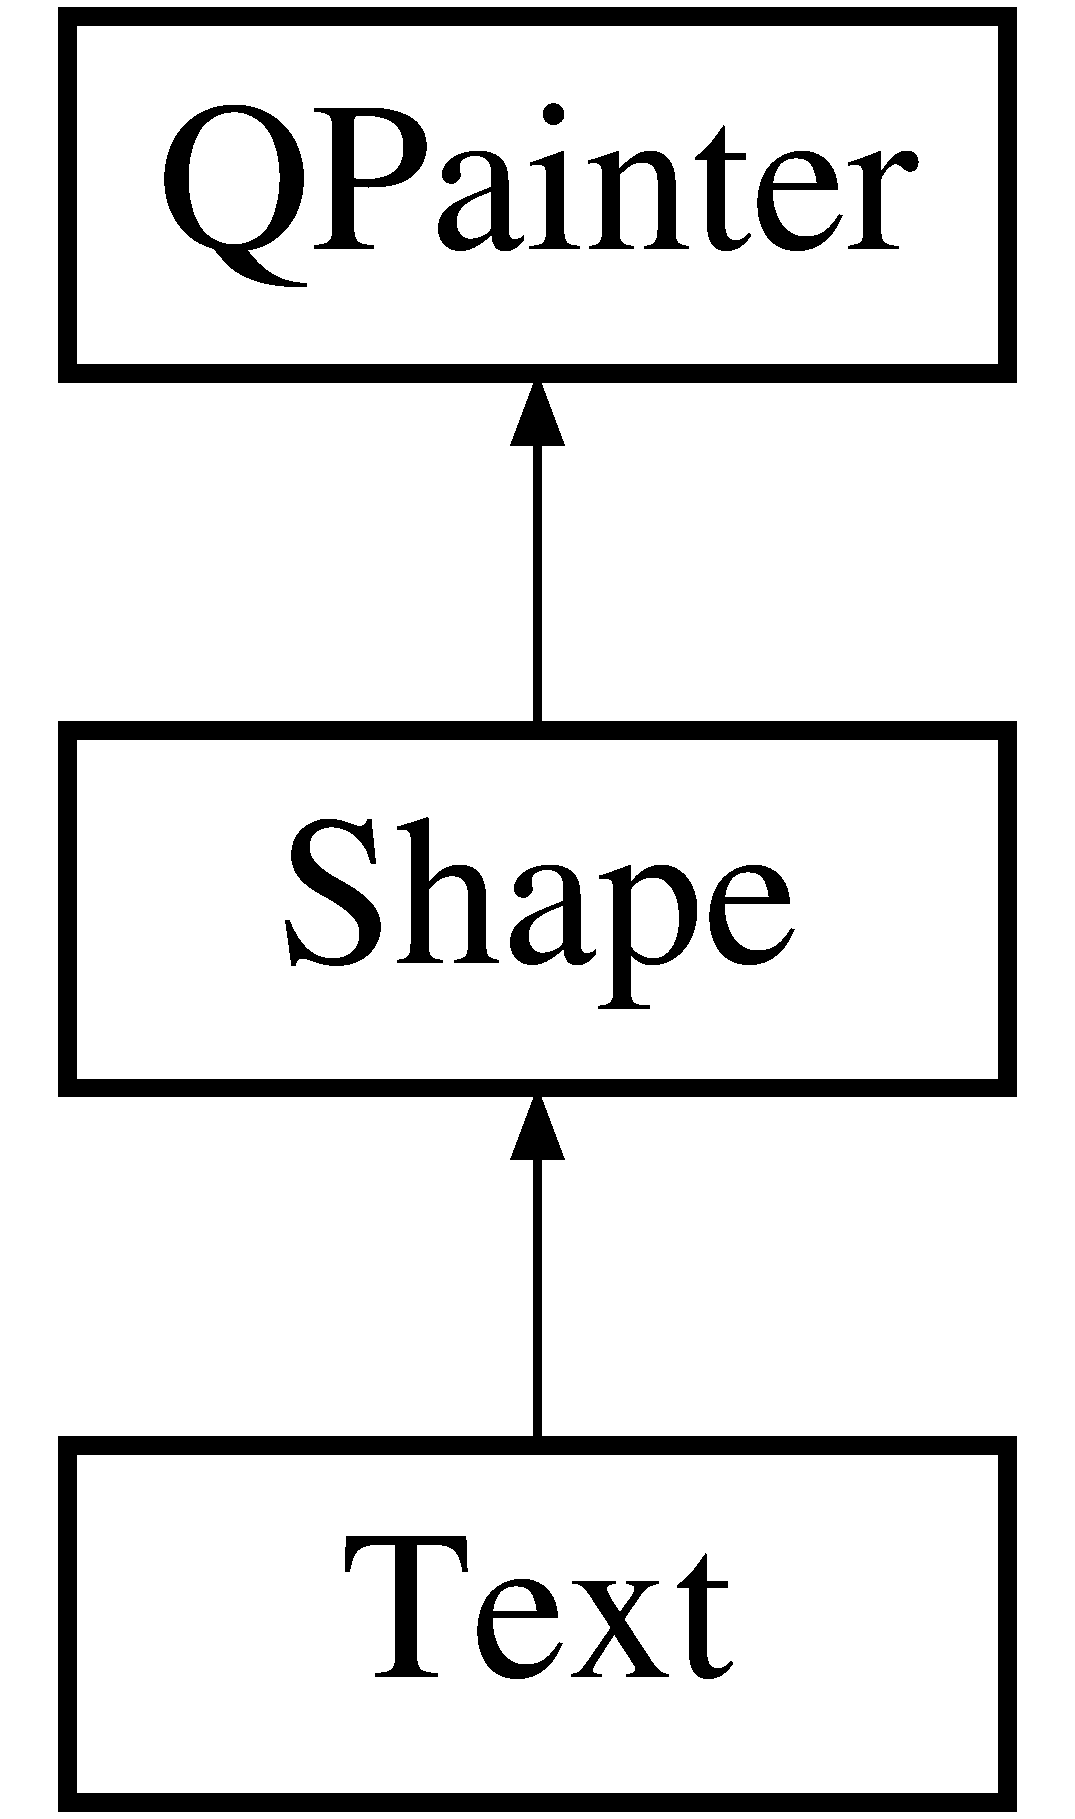
\includegraphics[height=3.000000cm]{class_text}
\end{center}
\end{figure}
\subsection*{Public Member Functions}
\begin{DoxyCompactItemize}
\item 
{\bf Text} (Q\+Paint\+Device $\ast$dev=nullptr, int id=-\/1)
\begin{DoxyCompactList}\small\item\em \doxyref{Text}{p.}{class_text} Class Constructor. \end{DoxyCompactList}\item 
void {\bf draw} (Q\+Paint\+Device $\ast$dev) override
\begin{DoxyCompactList}\small\item\em draw function to draw a text \end{DoxyCompactList}\item 
void {\bf move} (int x, int y, int junk) override
\begin{DoxyCompactList}\small\item\em move function to move a text \end{DoxyCompactList}\item 
double {\bf area} () override
\begin{DoxyCompactList}\small\item\em area function to calculate area of a text \end{DoxyCompactList}\item 
double {\bf perimeter} () override
\begin{DoxyCompactList}\small\item\em perimeter function to calculate permiter of a text \end{DoxyCompactList}\item 
void {\bf set\+Text} (Q\+String new\+Text)
\begin{DoxyCompactList}\small\item\em set\+Text function to set the font of the text \end{DoxyCompactList}\item 
void {\bf set\+Box\+Width} (int new\+Box\+Width)
\begin{DoxyCompactList}\small\item\em set\+Box\+Width function \end{DoxyCompactList}\item 
void {\bf set\+Box\+Height} (int new\+Box\+Height)\label{class_text_a7ecc194467d74cecff8b0027cb3534f5}

\begin{DoxyCompactList}\small\item\em set\+Box\+Height function \end{DoxyCompactList}\item 
void {\bf set\+Flag} (Qt\+::\+Alignment\+Flag flag)\label{class_text_af96574d035d39aaec84660de28dd9116}

\begin{DoxyCompactList}\small\item\em set\+Flag function \end{DoxyCompactList}\item 
void {\bf set\+Location} (int x, int y)
\begin{DoxyCompactList}\small\item\em set\+Location function for text \end{DoxyCompactList}\item 
void {\bf set\+Location} (Q\+Point pt)
\begin{DoxyCompactList}\small\item\em Set\+Location function for text. \end{DoxyCompactList}\item 
void {\bf set\+Dimensions} (int w, int h)
\begin{DoxyCompactList}\small\item\em set\+Dimensions function for text \end{DoxyCompactList}\item 
Q\+Font \& {\bf get\+Font} ()\label{class_text_aceef51d21bc54b84d040db42e425acd1}

\begin{DoxyCompactList}\small\item\em get\+Font function returns the font of the text. \end{DoxyCompactList}\item 
Qt\+::\+Alignment\+Flag {\bf get\+Flag} ()\label{class_text_abc42bd7502e8441a041f50695880bc8c}

\begin{DoxyCompactList}\small\item\em get\+Flag function returns the horizontal or vertical flag. \end{DoxyCompactList}\item 
Q\+String {\bf get\+Text} ()\label{class_text_a0315e3d6a80d496496838330e018e7e8}

\begin{DoxyCompactList}\small\item\em get\+Text returns the text object which provides a unicode character string. \end{DoxyCompactList}\end{DoxyCompactItemize}
\subsection*{Additional Inherited Members}


\subsection{Detailed Description}
\doxyref{Text}{p.}{class_text} Class\+: Public Inheritance From \doxyref{Shape}{p.}{class_shape} Class. 

\subsection{Constructor \& Destructor Documentation}
\index{Text@{Text}!Text@{Text}}
\index{Text@{Text}!Text@{Text}}
\subsubsection[{Text(\+Q\+Paint\+Device $\ast$dev=nullptr, int id=-\/1)}]{\setlength{\rightskip}{0pt plus 5cm}Text\+::\+Text (
\begin{DoxyParamCaption}
\item[{Q\+Paint\+Device $\ast$}]{dev = {\ttfamily nullptr}, }
\item[{int}]{id = {\ttfamily -\/1}}
\end{DoxyParamCaption}
)}\label{class_text_ae56225ea39562e2cc7b401b017d175b5}


\doxyref{Text}{p.}{class_text} Class Constructor. 

\doxyref{Text}{p.}{class_text} Class constructor takes in 2 arguments 
\begin{DoxyParams}{Parameters}
{\em $\ast$dev} & is a pointer of type Q\+Paint\+Device, initialized to nullptr to avoid conflict. \\
\hline
{\em id} & is of type int \\
\hline
\end{DoxyParams}


\subsection{Member Function Documentation}
\index{Text@{Text}!area@{area}}
\index{area@{area}!Text@{Text}}
\subsubsection[{area() override}]{\setlength{\rightskip}{0pt plus 5cm}double Text\+::area (
\begin{DoxyParamCaption}
{}
\end{DoxyParamCaption}
)\hspace{0.3cm}{\ttfamily [override]}, {\ttfamily [virtual]}}\label{class_text_ab9d0f9643d33550828eb23e3a5436036}


area function to calculate area of a text 

area function overrides the virtual area function of abstract base class shape. Function returns a double. No parameters are passed into area. 

Implements {\bf Shape} \doxyref{}{p.}{class_shape_aa3072fde001d5174f78fcc484c11870c}.

\index{Text@{Text}!draw@{draw}}
\index{draw@{draw}!Text@{Text}}
\subsubsection[{draw(\+Q\+Paint\+Device $\ast$dev) override}]{\setlength{\rightskip}{0pt plus 5cm}void Text\+::draw (
\begin{DoxyParamCaption}
\item[{Q\+Paint\+Device $\ast$}]{dev}
\end{DoxyParamCaption}
)\hspace{0.3cm}{\ttfamily [override]}, {\ttfamily [virtual]}}\label{class_text_a2401b42a363c41b8be6219eb1b14d08f}


draw function to draw a text 

draw function overrides the virtual draw from abstract base class shape. Funtion does not return any type. 
\begin{DoxyParams}{Parameters}
{\em $\ast$dev} & is a pointer of type Q\+Paint\+Device \\
\hline
\end{DoxyParams}


Implements {\bf Shape} \doxyref{}{p.}{class_shape_ad2ab549a1b0cc0e23af8be1fd1b61a1b}.

\index{Text@{Text}!move@{move}}
\index{move@{move}!Text@{Text}}
\subsubsection[{move(int x, int y, int junk) override}]{\setlength{\rightskip}{0pt plus 5cm}void Text\+::move (
\begin{DoxyParamCaption}
\item[{int}]{x, }
\item[{int}]{y, }
\item[{int}]{junk}
\end{DoxyParamCaption}
)\hspace{0.3cm}{\ttfamily [override]}, {\ttfamily [virtual]}}\label{class_text_af684963e401cbbddab1c3b5032e733bc}


move function to move a text 

move function overrides the virtual move from abstract base class \doxyref{Shape}{p.}{class_shape}. Function does not return any type. 
\begin{DoxyParams}{Parameters}
{\em x} & is of type int \\
\hline
{\em y} & is of type int \\
\hline
{\em junk} & is of type int \\
\hline
\end{DoxyParams}


Implements {\bf Shape} \doxyref{}{p.}{class_shape_a937ef09c5e1c5c640fdef7caf62ba8f2}.

\index{Text@{Text}!perimeter@{perimeter}}
\index{perimeter@{perimeter}!Text@{Text}}
\subsubsection[{perimeter() override}]{\setlength{\rightskip}{0pt plus 5cm}double Text\+::perimeter (
\begin{DoxyParamCaption}
{}
\end{DoxyParamCaption}
)\hspace{0.3cm}{\ttfamily [override]}, {\ttfamily [virtual]}}\label{class_text_aba53a89dd7a2fae148a403a8c4d2e9b1}


perimeter function to calculate permiter of a text 

perimeter function overrides the virtual perimter function of abstract base class shape. Function returns a double. No parameters are passed into area. 

Implements {\bf Shape} \doxyref{}{p.}{class_shape_afb064edd78952da66801619338e8c5a3}.

\index{Text@{Text}!set\+Box\+Width@{set\+Box\+Width}}
\index{set\+Box\+Width@{set\+Box\+Width}!Text@{Text}}
\subsubsection[{set\+Box\+Width(int new\+Box\+Width)}]{\setlength{\rightskip}{0pt plus 5cm}void Text\+::set\+Box\+Width (
\begin{DoxyParamCaption}
\item[{int}]{new\+Box\+Width}
\end{DoxyParamCaption}
)}\label{class_text_a83117073736a3c882180b46e9af22135}


set\+Box\+Width function 

set\+Box\+Width sets class member variable box\+Width to parameter new\+Box\+Width. 
\begin{DoxyParams}{Parameters}
{\em new\+Box\+Width} & is of type int \\
\hline
\end{DoxyParams}
\index{Text@{Text}!set\+Dimensions@{set\+Dimensions}}
\index{set\+Dimensions@{set\+Dimensions}!Text@{Text}}
\subsubsection[{set\+Dimensions(int w, int h)}]{\setlength{\rightskip}{0pt plus 5cm}void Text\+::set\+Dimensions (
\begin{DoxyParamCaption}
\item[{int}]{w, }
\item[{int}]{h}
\end{DoxyParamCaption}
)}\label{class_text_a4dfaf7c6694970dff0ff50f2205802da}


set\+Dimensions function for text 

set\+Dimensions function requires two parameters. The class member variables box\+Width and box\+Height are set from these parameters. 
\begin{DoxyParams}{Parameters}
{\em w} & is of type int \\
\hline
{\em h} & is of type int \\
\hline
\end{DoxyParams}
\index{Text@{Text}!set\+Location@{set\+Location}}
\index{set\+Location@{set\+Location}!Text@{Text}}
\subsubsection[{set\+Location(int x, int y)}]{\setlength{\rightskip}{0pt plus 5cm}void Text\+::set\+Location (
\begin{DoxyParamCaption}
\item[{int}]{x, }
\item[{int}]{y}
\end{DoxyParamCaption}
)}\label{class_text_a3d48c0d2794e52b4fa525d5d7e2ddf2f}


set\+Location function for text 

set\+Location function requires two arguments. Takes the two arguments and makes a coordinate pair consisting of these values. 
\begin{DoxyParams}{Parameters}
{\em x} & is of type int \\
\hline
{\em y} & is of type int \\
\hline
\end{DoxyParams}
\index{Text@{Text}!set\+Location@{set\+Location}}
\index{set\+Location@{set\+Location}!Text@{Text}}
\subsubsection[{set\+Location(\+Q\+Point pt)}]{\setlength{\rightskip}{0pt plus 5cm}void Text\+::set\+Location (
\begin{DoxyParamCaption}
\item[{Q\+Point}]{pt}
\end{DoxyParamCaption}
)}\label{class_text_a86d801852c8fe7d736915f2386b1134f}


Set\+Location function for text. 

set\+Location function requires a single parameter. The class memeber variable location is set to the Q\+Point parameter passed in. 
\begin{DoxyParams}{Parameters}
{\em pt} & is of type Q\+Point \\
\hline
\end{DoxyParams}
\index{Text@{Text}!set\+Text@{set\+Text}}
\index{set\+Text@{set\+Text}!Text@{Text}}
\subsubsection[{set\+Text(\+Q\+String new\+Text)}]{\setlength{\rightskip}{0pt plus 5cm}void Text\+::set\+Text (
\begin{DoxyParamCaption}
\item[{Q\+String}]{new\+Text}
\end{DoxyParamCaption}
)}\label{class_text_a9e7c48bfb75a9c2ddf246dc0a7add7e4}


set\+Text function to set the font of the text 

set\+Text requires a Q\+String parameter 
\begin{DoxyParams}{Parameters}
{\em new\+Text} & is of type Q\+String \\
\hline
\end{DoxyParams}


The documentation for this class was generated from the following file\+:\begin{DoxyCompactItemize}
\item 
Shape.\+h\end{DoxyCompactItemize}

%--- End generated contents ---

% Index
\backmatter
\newpage
\phantomsection
\clearemptydoublepage
\addcontentsline{toc}{chapter}{Index}
\printindex

\end{document}
